% ==== BEGIN OF PREAMBLE =======================================================
% ---- document class (use appropriate driver for DIV to PS/PDF conversion):
\documentclass[12pt,a4paperx]{book}


% ---- graphicx package:
\usepackage{graphicx}


% ---- natbib package:
\usepackage{natbib}
\bibpunct{(}{)}{;}{a}{}{,}  % adjust author-year citation format 


% ---- hyperref package for cross-references:
\usepackage{hyperref}
% -- USE BLACK LINKS IN PRINTOUT (uncomment the following lines if necessary):
%\hypersetup{colorlinks,%
%            linktocpage,%
%            breaklinks,%
%            citecolor=black,%
%            filecolor=black,%
%            linkcolor=black,%
%            urlcolor=black,}
% -- use color links in pdf version (comment the following lines if necessary):
\hypersetup{colorlinks,
            linktocpage,%  make page number, not text, be link on TOC, LOF & LOT
            breaklinks,%
            citecolor=blue,%
            filecolor=blue,%
            linkcolor=blue,%
            urlcolor=blue,}


% ---- caption package:
\usepackage[font=small,labelfont=bf]{caption}


% ---- subfigure package:
\usepackage[tight,nooneline,FIGTOPCAP,bf]{subfigure}
% \setlength{\subfigcaptopadj}{-6pt}  % vertical position of subfigure labels
\renewcommand{\thesubfigure}{\alph{subfigure}}
\makeatletter
    \renewcommand{\@thesubfigure}{(\thesubfigure)}  % subfigure labels:     (a)
    \renewcommand{\@@thesubfigure}{\thesubfigure}   % produced by \subref:   a
    \renewcommand{\p@subfigure}{\thefigure}         % produced by \ref:   3.1a
\makeatother


% ---- fancyhdr package:
\usepackage{fancyhdr}


% ---- some other useful packages:
% \usepackage{showkeys}  % show all keys (labels)
% \usepackage{times}     % use times new roman instead of computer modern font


% ---- page layout:
\setlength{\textheight}{24cm}
\setlength{\textwidth}{15cm}
\setlength{\topmargin}{-0.9cm}
\setlength{\headheight}{0.6cm}
\setlength{\headsep}{1cm}
\setlength{\footskip}{1cm}
\setlength{\oddsidemargin}{9.1mm}
\setlength{\evensidemargin}{-0.2mm}
\setlength{\marginparwidth}{2cm}


% ---- paragraph and line properties:
\setlength{\parindent}{0.8cm}
\setlength{\parskip}{0pt}
\linespread{1.2}
\sloppy % reduce number of word divisions and use more space between words


% ---- header format: use fancyhdr page style:
\pagestyle{fancy}
\fancyhf{}
\renewcommand{\chaptermark}[1]{\markboth{#1}{}}
\renewcommand{\sectionmark}[1]{\markright{\thesection\ #1}}
\fancyhead[LE,RO]{\thepage}
\fancyhead[LO]{\slshape \small \rightmark}
\fancyhead[RE]{\slshape \small \leftmark}
\renewcommand{\headrulewidth}{0pt}


% ---- define label format for equations, figures, and tables:
\renewcommand{\theequation}{\thechapter.\arabic{equation}}
\renewcommand{\thefigure}{\thechapter.\arabic{figure}}
\renewcommand{\thetable}{\thechapter.\arabic{table}}


% ==== END OF PREAMBLE =========================================================


% ==== BEGIN OF BODY ===========================================================
\begin{document}


% ==== START FRONT MATTER (use ROMAN numerals) =================================
\frontmatter


% ==== TITLE PAGE ==============================================================
% ---- include tex-file (CHOOSE APPROPRIATE FILE):
\begin{titlepage}
\begin{center}

% ---- main title
~\\[15mm]
{\Huge  {\bf Estimating Glaciers Ice Thickness with Machine Learning}}\\[5mm]


% ---- subtitle (if necessary):
%{\LARGE {\bf Scientific Writing in \LaTeXe{}}}\\[15mm]


% ---- type of thesis:
{\Large \textsc{Master's Thesis}} \\[15mm]


% ---- field of study:
{\large in Atmospheric Sciences} \\[15mm]


% ---- institution:
{\large Submitted to the} \\[2mm]
{\Large \textsc{Faculty of Geo- and Atmospheric Sciences}} \\[2mm]
{\large of the} \\[2mm]
{\Large \textsc{University of Innsbruck}} \\[15mm]


% ---- degree:
{\large in Partial Fulfillment of the Requirements for the Degree of} \\[2mm]
{\Large \textsc{Master of Science}} \\[15mm]


% ---- author:
{\large by} \\[2mm]
{\Large \textsc{Matteo Castellani}} \\[15mm]


% ---- advisor:
{\large Advisor} \\[2mm]
{\large Assistant Professor Dr. Fabien Maussion} \\[15mm]


% ---- location, date:
{\large Innsbruck, March 2020}


\end{center}
\end{titlepage}
    % activate this line for Master's Thesis
% \begin{titlepage}
\begin{center}

% ---- main title
~\\[15mm]
{\Huge  {\bf A Template for a Science Thesis:}}\\[5mm]


% ---- subtitle (if necessary):
{\LARGE {\bf Scientific Writing in \LaTeXe{}}}\\[15mm]


% ---- type of thesis:
{\Large \textsc{Diploma Thesis}} \\[15mm]


% ---- field of study:
{\large in Meteorology} \\[15mm]


% ---- institution:
{\large Submitted to the} \\[2mm]
{\Large \textsc{Faculty of Geo- and Atmospheric Sciences}} \\[2mm]
{\large of the} \\[2mm]
{\Large \textsc{University of Innsbruck}} \\[15mm]


% ---- degree:
{\large in Partial Fulfillment of the Requirements for the Degree of} \\[2mm]
{\Large \textsc{Master of Natural Science}} \\[15mm]


% ---- author:
{\large by} \\[2mm]
{\Large \textsc{FirstName LastName}} \\[15mm]


% ---- advisor:
{\large Advisor} \\[2mm]
{\large Univ.-Prof. Dr. Hans Ertel} \\[15mm]


% ---- location, date:
{\large Innsbruck, December 2009}


\end{center}
\end{titlepage}
   % activate this line for Diploma Thesis
\newpage
~\thispagestyle{empty}
\newpage
% ---- start page numbering again:
\setcounter{page}{1}


% ==== DEDICATION ==============================================================
% ---- include tex-file:
% \addcontentsline{toc}{chapter}{Dedication}
\thispagestyle{plain}

\begin{center}
 \Large\em\null\vskip5cm To Lisa and the Rolling Stones \\[3cm]
\end{center}

\newpage
\thispagestyle{plain}


% ==== PREFACE =================================================================
% ---- include tex-file:
\chapter*{Preface}
\addcontentsline{toc}{chapter}{Preface}
\thispagestyle{plain}

This \LaTeXe{} template is based on my own dissertation. It has been extensively
modified within the framework of the course \emph{Introduction to Scientific
Working} which I taught at the University of Innsbruck in the winter semester
2009/2010 for students of the \emph{Atmospheric Sciences Master Program}. It
does \emph{not} serve as the official thesis template of the Institute of
Meteorology and Geophysics (IMGI), however, it follows some reasonable rules,
such as the reference and citation guidelines of the American Meteorological
Society. Before using this template at IMGI, make yourself familiar with the
format guidelines of the Faculty of Geo- and Atmospheric Sciences and
the personal preferences of your advisor. My \LaTeX{} knowledge is based on the
guides of \citet{oeti08Aag} and \citet{kopk99Aag}. Many ideas on the content and
structure of a science thesis are taken from the book of \citet{russ06Aag}. This
template is distributed in the hope that it will be useful, but \emph{without
any warranty}. I am looking forward to receiving comments for
improvements.\footnote{\texttt{alexander.gohm [at] uibk.ac.at}}

\begin{flushright}
\textit{Alexander Gohm}

\textit{Innsbruck, December 2009} 
\end{flushright}

\newpage
\thispagestyle{plain}


% ==== ABSTRACT ================================================================
% ---- set some counters to zero:
\setcounter{equation}{0}
\setcounter{table}{0}
\setcounter{figure}{0}
% ---- include tex-file:
\chapter*{Abstract}
\addcontentsline{toc}{chapter}{Abstract}
\thispagestyle{plain}

The abstract is a short summary of the thesis. It announces in
a brief and concise way the scientific goals, methods, and most important
results. The chapter ``conclusions'' is not equivalent to the abstract!
Nevertheless, the abstract may contain concluding remarks. The abstract
should not be discursive. Hence, it cannot summarize all aspects of the thesis
in very detail. Nothing should appear in an abstract that is not also
covered in the body of the thesis itself. Hence, the abstract should be the
last part of the thesis to be compiled by the author.

A good abstract has the following properties: \emph{Comprehensive:} All major
parts of the main text must also appear in the abstract. \emph{Precise:}
Results, interpretations, and opinions must not differ from the ones in the main
text. Avoid even subtle shifts in emphasis. \emph{Objective:} It may contain
evaluative components, but it must not seem judgemental, even if the thesis
topic raises controversial issues. \emph{Concise:} It should only contain the
most important results. It should not exceed 300--500 words or about one page.
\emph{Intelligible:} It should only contain widely-used terms. It should
not contain equations and citations. Try to avoid symbols and acronyms (or at
least explain them). \emph{Informative:} The reader should be able to quickly
evaluate, whether or not the thesis is relevant for his/her work.

An Example: The objective was to determine whether \dots (\emph{question/goal}).
For this purpose, \dots was \dots (\emph{methodology}). It was found that \dots
(\emph{results}). The results demonstrate that \dots (\emph{answer}).

\newpage
\thispagestyle{plain}


% ==== TABLE OF CONTENTS =======================================================
~
\newpage
\addcontentsline{toc}{chapter}{Contents}
\tableofcontents
\newpage
\thispagestyle{plain}


% ==== START MAIN MATTER (use ARABIC numerals) =================================
\mainmatter


% ==== INTRODUCTION (CHAPTER 1) ================================================
% ---- set some counters to zero:
\setcounter{equation}{0}
\setcounter{table}{0}
\setcounter{figure}{0}
% ---- include tex-file:
\chapter{Introduction}\label{chap1}
\thispagestyle{plain}

% ====SECTION 1 ================================================================
\section{Motivation}\label{motivation}
Estimating the volume of glaciers is becoming an increasingly important topic, due to the role this plays in climate change. Melting glaciers have in fact an impact in sea level rise \citep{Zemp2017}, availability of fresh drinking water \citep{Kaser2010}) and even energy supplied by hydro electric power plants\citep{Terrier2011}. A reliable estimate of glaciers volume is key in order to properly compute the entity of these and other problems.

Computing the volume of glaciers is a trivial task once in possession of the data needed for it: the glacier surface and its distributed ice thickness. These data however are not easily obtainable due to the amount of effort needed to collect them.

A very big effort in this regard has been carried out with the creation of the Randolph Glacier Inventory (RGI) \citep{RGI2014}, which is a data-set containing a globally complete inventory of glaciers and their surface shapes. From these surface shapes it is easy to compute the surface area of the glaciers.

Ice thickness observations are collected in the Glacier Thickness Database (GlaThiDa) \citep{GlaThiDa2014}, which is the first global effort in collecting all the available ice thickness data in a single database. These observations however, when compared with the glaciers contained in the RGI, are very sparse (see \ref{glathida}). Out of the over 215,000 glaciers included in RGI, only 771 have thickness observations and, for most glaciers, there are not enough measurements to have a complete thickness distribution along the glacier surface. 

Modeling glaciers is the only alternative to obtain an estimate of their volumes and is where a big effort from the scientific glaciology community is directed.
  
%The chapter Introduction leads the reader into the subject matter
%of the thesis. It is sometimes called
%Statement/Formulation/Definition/Presentation of the Problem. It may start with
%a so-called Motivation. It also contains the State of Knowledge or State
%of Research which is based on a literature survey (see section \ref{1sec:2}).
%Further, it contains the Scientific Questions and/or the Goals that are
%addressed in the main part of the thesis (see section \ref{1sec:3}). Finally,
%it provides an Outline of the science thesis (see end of section \ref{1sec:3}). 


% ==== SECTION 2 ===============================================================
\section{State of Research}\label{research}
Over the years a number of different approaches have been used to model glaciers and estimate their volumes.
The simplest ones only attempt to compute these volumes from the relationship between the glacier surface and its volume as first stated by \citet{bahr1997}. Using the Buckingham Pi
theorem they found that the relationship between the surface area $S$ and the volume of a glacier $V$ is $V \propto S^{\gamma}$ and they estimated $\gamma=1.375$ for these glaciers and $\gamma=1.25$ for ice caps. Similar approaches also take into consideration other other parameters such as glacier length, width, elevation range \citep{Grinsted2013}, and surface slope. These type of methods are called ``scaling approaches'' and they yield to a volume estimate for each glacier but not to the distributed ice thickness. Due to the small requirements for their implementations they are very effective at computing the global volume of glaciers.

A more sophisticated approach to estimate the volume of glaciers is to reconstruct their three dimensional shape with a model, and thus calculate the volume. Traditionally this is done by making physical assumptions about the glacier dynamics and solving equations deriving from these assumptions to estimate the glacier shape. Numerical methods are then used to obtain a discretization of these equations which are then solved on grid-cell maps by computers. This set of numerically solved equations are what composes the model. 
For glaciers this means reconstructing their bed shapes from their surface values, hence inverting the bed shape from the surface measurements using the constructed model.
 

%The equations needed to create the glacier map depend on parameters which are often unknown. This creates the inverse problem of having to estimate these parameters from observed data. In the case of estimating the glacier ice thickness to compute its volume, the problem would then be to tune the model parameters of the numerically solved equations, to best reproduce the observed ice thickness.  
%These equations depend on parameters which need to be tuned in order for the equations to replicate the available observations. The tuning of these parameters is known as the inverse problem which needs to be solved in order for the  In the case of the    This can be done starting from te known values of the glaciers surface such as the glacier shape, available in the RGI, and the topography of the glacier, obtainable from a digital elevation model. This leads to a grid-map containing the glacier surface shape and the elevation of each grid point. Using these and potentially other values such as the glacier climate, one could create an algorithm based on physical assumptions or statistical data, to estimate the bed shape of the glacier. able to numerically compute the glacier bed shape using either a physical or statistical numerical   and extrapolate the volume from the results of this simulation. Usually physical assumptions must be made to be able to reproduce the glacier bed from its surface ice distribution.
First steps in this direction were made by \citet{Nye1965} in the study of  idealized glaciers. He pointed out that the distributed ice thickness could be inferred by the glacier surface slope using estimates of basal shear stress. From there many others developed this idea, such as \citet{haeberli1995} who made the assumption of a known constant basal shear stress, parameterized from the glacier elevation range, to estimate basic glaciological characteristics for glaciers in the Alps. 

From these basic concepts, many more approaches have emerged in the years after, taking for example the mass conservation into account \citep{rasmussen_1988}, basal slipperiness together with bedrock topography \citep{Gudmundsson2001}, information such as mass balance and surface velocities (e.g. \citealt{gantayat2014}, \citealt{brinkerhoff2016}) and even more complex ones using forward models of ice flow \citep{vanPelt2013}. Also some non physical methods such as artificial neural networks \citep{Clarke2009}, have been adopted all to tackle the problem of estimating glaciers ice thickness. 

All these achievements have been possible thanks to the advancement in research in the glaciological field and to the steadily increase in computational power and its availability. Models which could only be numerically computed for single glaciers, started expanding their range of possibilities, and \citet{Huss2012} released the first glacier model used to model all known glaciers and ice caps worldwide. Since then many more global scale glacier models able to predict ice thickness distribution have been released. 

Meanwhile the GlaThiDa database was being compiled. This is a a collection of in-situ observations of glaciers ice thickness, created by joining together in a single database all the available ice thickness observations from worldwide glaciers. In particular it contains a table listing point-wise ice thickness measurements and their geographical coordinates. Even though these data are far from being enough to obtain ice volume estimates for all glaciers in the world, they are very useful for assessing glacier models performances. 

The compilation of GlaThiDa together with the increase number of models being adopted by the glaciology community led to the first Ice Thickness Models Intercomparison eXperiment (ITMIX) \citep{Farinotti2017}, which is the first attempt to put together all those models and asses their accuracy on the base of known ice thickness observations available in the GlaThiDa, as well as comparing the models performances with each other. 

The experiment focused on 17 glacier models which were given the task to estimate the ice thickness distribution of at least some of 15 glaciers, 3 ice caps and 3 synthetically grown glaciers. In order to predict the ice thickness the models were not allowed to use ice thickness observations for calibration. The output of the models was then compared with data available from the GlaThiDa and with the other models. A composite solution from all the participating models achieved a local ice thickness difference in the order of $10 \pm 24\%$ of the mean ice thickness. In general however the spread of the solutions obtained by the single models often exceeded the local ice thickness, concluding that an ensemble approach could mitigate errors and would reduce the random nature of single models output.  

The models participating in the ITMIX were divided into categories depending on the different approaches used to model the ice thickness. The categories are: (1) those taking ice thickness inversion approaches as a minimization problem, (2) those based on mass conservation,  (3) approaches depending on a basal shear stress parametrization, (4) approaches based on surface velocities and (5) other approaches. 15 out of the 17 explored models in the ITMIX, belong to the first 4 categories, which are all categories for methods relaying on physical assumptions to model numerically some of the physical processes happening in a glacier and predict the ice thickness from there. Only 2 models, belonging to category (5) are models not based on physical assumptions and methods, but rather on statistical methods. Of those two the one from \citet{Clarke2009} is based on artificial neural networks, a branch of machine learning. It uses the input data from artificially grown glaciers to make predictions about real glaciers ice thickness, learning from the input data of the artificially grown ones. At the time of Clarke's publication in fact the GalThiDa had not yet been compiled, and there were not enough ice thickness observations available, to train a machine learning model from real glacier data.

Machine learning is a branch of computer science which uses different algorithms to give a computer the ability to learn from a set of samples. The concept of artificial intelligence, which is the super field of machine learning, was first proposed by \citet{Turing1950}.

Many different machine learning algorithms have been developed since 1950 and some even before. Although the algorithms have been around for a long period of time, they only saw wide spread application starting from the late 1990, as computation power and resources largely improved. Since then however the field has seen a huge development and many of its applications have become part of our day to day life. Things such as voice recognition, chat bots, autonomous driving and online products suggestions, are all a products of machine learning algorithms being developed and trained to solve these specific problems.

The basic idea behind machine learning is to allow a computer program to generate a model capable of solving a task, without explicit instructions on how to solve it. In the case of the glacier thickness it would mean to feed the algorithm a data sample including observed glacier ice thicknesses, to learn form possible patterns within this sample. After the learning process is finished one could use the trained model (as algorithms which underwent the learning process are called) to make predictions about glaciers with no thickness observations, or to fill the holes for those with too few ones.

Machine learning however has yet to make a big impact in the glaciological community and most of the models used in the ITMIX, and the ones which achieved better accuracy, are physically based models. In a later experiment, \citet{Farinotti2019} (F19) developed an ensemble model, using 5 of the physically based models form the first ITMIX, to better predict ice thickness distributions of all glaciers in the world. The results from this experiment can be used as good benchmark to compare models based on machine learning algorithms.

The importance glaciers play in climate change and climate modeling, the availability of ice thickness observations, the excitement behind machine learning in almost every possible field, and the lack of previous work done in this sense by the glaciological modeling community, are the driving motivation factors for this thesis.

%Based on the literature survey, the writer draws a picture of the existing
%knowledge in a specific field and points to open questions. Hence, after this
%survey the Introduction will ultimately culminate in the formulation of specific
%scientific questions/goals addressed in the thesis (see section \ref{1sec:3}).

%To cite a certain source (e.g., a paper) use the citation commands
%\verb|\citet| and \verb|\citep| of the \verb|natbib|
%package.\footnote{
%\url{http://www.ctan.org/tex-archive/macros/latex/contrib/natbib/natnotes.pdf}}
%Together with the bibliography style \verb|ametsoc.bst|, which is
%included in the \LaTeX{} manuscript template for AMS journals\footnote{
%\url{http://www.ametsoc.org/PUBS/journals/AMS_Latex_V3.0.tar.gz}}, \verb|natbib|
%produces citations in the author-date format together with a list of
%references that fulfill the AMS citation standard.\footnote{
%\url{http://www.ametsoc.org/PUBS/journals/author_reference_guide.pdf}}
%
%As an example, you can cite papers like \citet{hann66Aag} and \citet{scha93Aag}
%which have to be specified in your BibTeX database file (in this case it is
%\verb|mybibfile.bib|). More than one article of the same author can be cited
%like here: \citet{hoin85Aag,hoin90Aag} studied foehn winds.
%
%You may want to split your review of the literature into several sections.
%Further, use paragraphs to structure your introduction. If you like to cite
%papers in brackets (\emph{passive citations}) you can do this
%as in the following sentence: Gap flows have been studied in the Strait
%of Gibraltar \citep{scor52Aag,dorm95Aag}, in the French Rh\^one Valley
%\citep{pett82Aag}, near Hokkaid\=o in Japan \citep{arak69Aag}, near
%Unimak Island in the Aleutian Chain \citep{pan-99Aag}, and in the Howe
%Sound of British Columbia \citep{jack94Aag,jack94Bag}. Citation of a
%Dissertation: The gap flow in the Wipp Valley has been studied by
%\citet{gohm03Aag}. Citation of a conference paper: \citet{gohm06Aag}
%investigated the boundary layer structure in the Inn Valley. Citation of an
%online document: The AMS provides a guideline for preparing citations and
%references \citep{ams-09Aag}.


% ==== SECTION 3 ===============================================================
\section{Goals and Outline}\label{goals}
In this thesis three different machine learning algorithms have been chosen to  create models able to predict glacier ice thickness. The algorithms have all been trained on the same data-set, the GlaThiDa which contains ice thickness observations for glaciers worldwide.

To train the algorithm a set of attributes (often called features), mainly geometrical, have been generated using the Open Global Glacier Model (OGGM) \citep{OGGM2019}. This attributes are all computable by the only mean of a digital elevation model for the considered glacier, and the outline of the glacier given by the RGI.

The accuracy of the models have been estimated comparing their predictions with the observations from the GlaThiDa as well as with themselves.

An analysis of the most influential attributes in making predictions has been carried out.

Finally the obtained models have been used to predict the volume of all the alpine glaciers and compare their results with those of the \citet{Farinotti2019} (F19).


This thesis then tries to establish:
\begin{itemize}
\item[(1)] How accurate machine learning algorithms are at predicting glaciers ice thickness.
\item[(2)] How three different machine learning algorithms compare with each other in estimating glaciers ice thickness.
\item[(3)] Using those algorithm to estimate the total volume of glaciers in the alps, how these models compare to the model from the \cite{Farinotti2019} (F19).
\end{itemize}

%The so-called SMART
%criteria\footnote{\url{http://en.wikipedia.org/wiki/SMART_criteria}} might be
%used as a guideline to define reasonable goals. Here, the acronym SMART
%describes the properties of ``good'' goals: \underline{s}pecific,
%\underline{m}easurable, \underline{a}ttainable, \underline{r}elevant,
%\underline{t}ime-bound.
%
%The introduction may also describe briefly the methodology chosen and the
%materials (e.g., data, instruments, etc.) used. However, a detailed description
%will follow in the main part (see chapter \ref{chap2}).
%
%Finally you should present an \emph{outline} of your science thesis. Explain
%what the reader will find in the following chapters. For example, chapter
%\ref{chap2} describes the methodology. The results are presented
%in chapter \ref{chap3}. A discussion is provided in chapter \ref{disc} and the
%conclusions are drawn in chapter \ref{concl}.

\newpage
\thispagestyle{plain}


% ==== CHAPTER 2 ===============================================================
% ---- set some counters to zero:
\setcounter{equation}{0}
\setcounter{table}{0}
\setcounter{figure}{0}
% ---- include tex-file:
\chapter{Methodology}\label{chap2}
\thispagestyle{plain}

%This chapter provides a detailed description of the methodology. It is
%sometimes called Experimental Section. Depending on the subject it is a
%``synonym'', e.g., for Theoretical Section, Computational Methods, Model
%Description and Setup, Field Work, and so on. Hence, this chapter contains a
%description of \emph{what has been done} in order to address the scientific
%question raised in the chapter Introduction. However, it does \emph{not} contain
%the results! 


% ==== SECTION 1 ===============================================================
%\section{Experimental Set-up}\label{2sec:1}
%Depending on the topic of the science thesis, this chapter may contain a
%description of the experimental set-up, the field experiment,
%datasets, instruments, measurement procedures, analysis techniques, calibration
%and quality control, and other things. In case of a modeling study it may
%contain the formulation and derivation of model equations, the formulation of
%initial and boundary conditions, the data used to drive and validate the model,
%an overview of the model set-up (e.g., parameter set-up), modifications of the
%``original'' model code, a description of relevant parameterizations,
%a theoretical background needed for the interpretation of model results.


% ==== SECTION 2 ===============================================================
\section{Data Sets}\label{glathida}
This section gives an overview of the data used in the analysis done in this thesis. The basics data to run all the analysis have been the Glacier Thickness Database (GlaThiDa), the Randolph Glacier Inventory (RGI), and different digital elevation models (DEMs) which are dependent on the specific glacier. Depending on the region in fact some digital elevation models are a better fit to each glaciers as all of the freely available ones have missing data. ``The best'' digital elevation model has been automatically chosen by the Open Global Glacier Model (OGGM). Through most of the analysis SRTM v4 (\citet{SRTM}) which is a 90m grid resolution DEM has been used. Other DEM might have been used to link the GlaThiDa with RGI (see section \ref{GlaRGI})

\subsection{GlaThiDa}
The glacier Thickness Database (\citet{GlaThiDa2014}) is a set of data which attempts to put together all the available ice thickness measurements from glaciers and ice caps all around the globe. The database is composed of three different tables. The first one contains an overview of the database, the second one thickness data from maps or digital elevation models (DEM), and the third one, the one used in this thesis, contains the actual point measurements with the thickness data. The measurements were taken with different methods such as terrestrial and airborne radio-echo sounding, ground penetrating radar, direct drilling and other methods. The first database was released in 2014. In 2016 a second version 2.0 and its correction 2.1 were released, and in 2019 version 3.0 and 3.01 were finally released. All the analysis in this work have been done using version 2.1 as version 3.0 was released after a big part of the analysis was already done. According to the \href{https://github.com/ezwelty/glathida/blob/master/CHANGELOG.md}{change log} however most of the changes have been done to the structure of the data base. There were however some measurements additions to the database. The addition of some measurements for some glaciers in Switzerland in particular would be relevant for this thesis, given that most of the analysis done in this work has been conducted over the alpine glaciers. 
%Use subsections to structure your thesis. The first and second component of the
%momentum equation is shown in equation (\ref{2equ:1}) and (\ref{2equ:2}),
%respectively. Together with (\ref{2equ:3}) they form the set of shallow-water
%equations implemented in a numerical model.

\subsection{RGI}
The Randolph Glacier Inventory (RGI) (\citet{RGI2014}) is a global database of outlines of glaciers, excluding ice sheets. The inventory has been compiled from satellite imagery collected from 1999 onward. Most of the outlines don't express a specific picture in time of the glacier but are a compound of different images of each glacier due to images obstructions such as cloud covers or satellite orbits. The first version of this inventory was released in 2012 and the latest version, RGI Version 6.0 was released in 2017. In this latest release the database comprises more than 220,000 glacier outlines which are divided in 19 regions which cover all areas in the world with glaciers. This is the version used for all the analysis in this thesis. \todo{Add map of all the glaciers?}

\subsection{Linking GlaThiDa and RGI}\label{GlaRGI}
The GlaThiDa comes with a table containing the thickness measurements observations. This table comes with the thickness value of the observation, its latitude and longitude, and other variables such as the date of the observation, the name of the glacier, the thickness uncertainty and others. Aside from the measurements GPS coordinates and the thickness value, some fields like, the name of the glacier and the thickness uncertainty, are often left empty. This creates the problem of having to link each observation with a glacier in the RGI database. To do so a script has been created which determines whether an observation is located inside a glacier outline: the RGI database comes with closed outlines of the glaciers in geographic coordinates referenced to the WSG84 (also known as ESPG:4326) as shape-files. The python library \href{https://github.com/Toblerity/Shapely}{shapely} has been used to transform the observation Latitude and Longitude to the WSG84 projection system and to check whether each of these point was lying inside the glacier outlines (including the boundaries of the outline).
\todo{Add graphic of a glacier with the thickness points. I couldn't find a script with it so far.}

\subsection{Some statistics about GlaThiDa}
After linking the two databases it is interesting to learn about some statistics of the GlaThiDa. In order to create these statistics The Open Global Glacier Model (OGGM) (\citet{OGGM2019}, \href{https://github.com/OGGM/oggm}{Open Source Code}) has been used to add a digital elevation model to the glaciers in the RGI with thickness entries in the GlaThiDa (see \ref{GlaRGI}).

\subsubsection{Glaciers distribution and types}
There are 820370 entries (thickness measurements) in the GlaThiDa version 2.1. After assigning each of them to one of the 215,547 RGI glaciers 771 of those glaciers have thickness observations associated with them. This is 0.36\% of all the glaciers in th RGI. Out of the 820370 initial entries 27882, 3.4\% resulted outside of any glacier outlines defined in the RGI. Some reason for this could be: a slightly wrong GPS coordinate collected in the GlaThiDa measurement; observations taken outside of the glacier by mistake or intentionally, to make sure that all the glacier was covered; a different shape of the glacier at the moment when the observation was taken, compared to the moment when the RGI was compiled; a wrong assessment of the glacier shape in the RGI.
\begin{figure}\label{glathidamap} 
	\centering 
	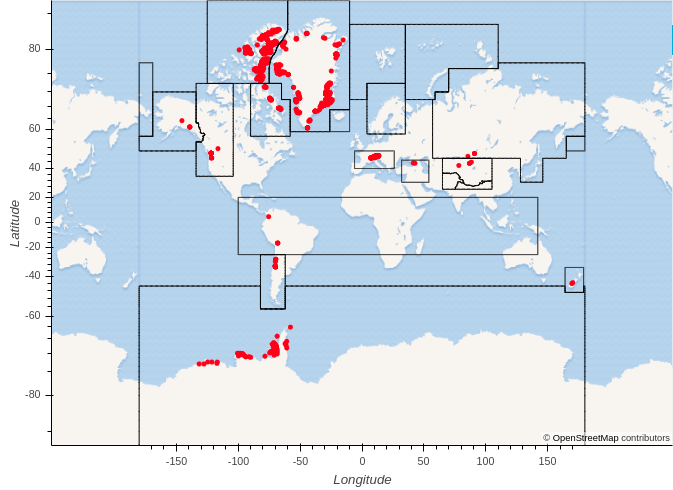
\includegraphics[width=1.0\textwidth]{./figures/GlaThiDa_map.png}
	\caption{Global map of the distribution of glaciers with thickness observations entries in the GlaThiDa database version 2.1. Black outlines are the RGI regions.}
\end{figure}

Most of the glaciers with thickness observation are in the Greenland Periphery region and in the Artic Canada North region. If we compare the glaciers with measurements with the number of glaciers present in each specific region though, we see that Arctic Canada North is the best represented region with around 5\% of the glaciers having at least one thickness measurement point. The region with most glaciers, Central Asia, has a very low number of glaciers represented in the GlaThiDa database. This is probably due to the difficulty in getting measurements for glaciers as such high altitudes at those present in the Himalaya.


\begin{figure}[!tp]
	\centering		  
	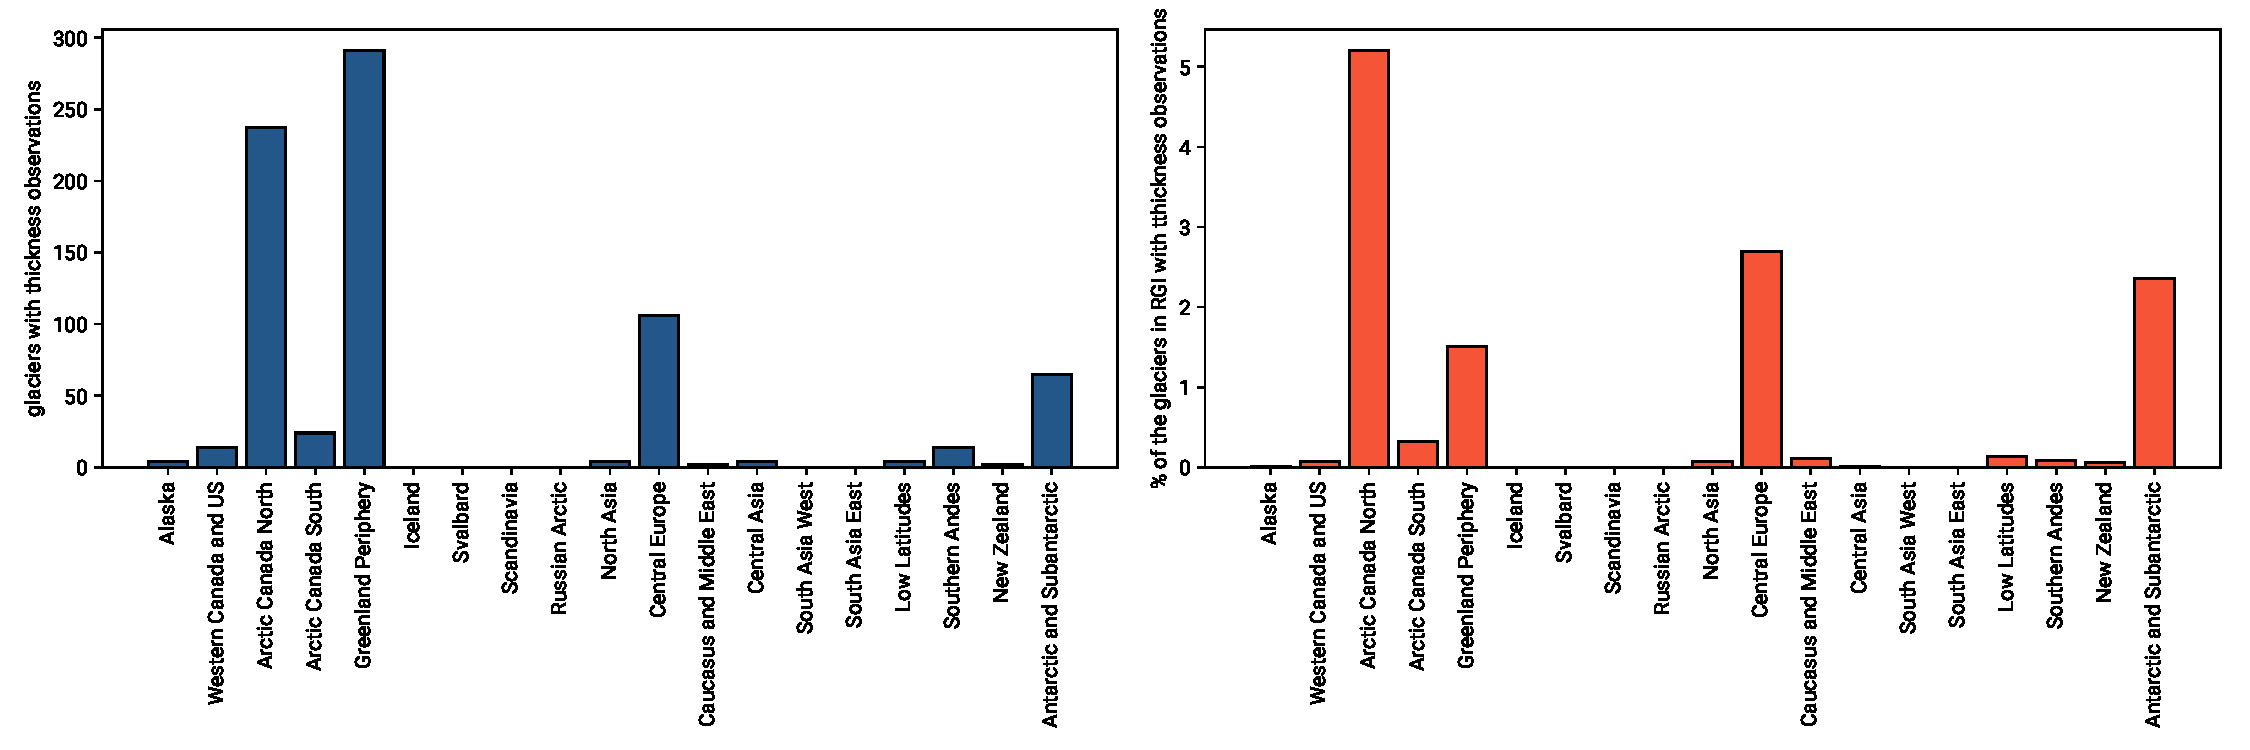
\includegraphics[width=1.\textwidth]{figures/Observations_per_region.pdf}
	\caption{On the left side the number of glaciers in the RGI with thickness observations in the GlaThiDa are shown per RGI region. On the right side the percentage of glaciers for each region with thickness observations is shown instead.}
	\label{fig:glareg}
\end{figure}

More than two third of the RGI entities with GlaThiDa measurements are glaciers while the rest are ice caps. Land terminating glaciers and ice caps are the vast majority.

\subsubsection{Measurements Distribution per Glacier}
Not all the glaciers with measurements are perfectly covered over the whole glacier area. In fact around 42\% of the glaciers have less than 100 thickness observations. Given that some glaciers can extend for over $100 km^2$, it’s clear that some of them are very poorly covered.
\begin{figure}[!tp]
	\centering		  
	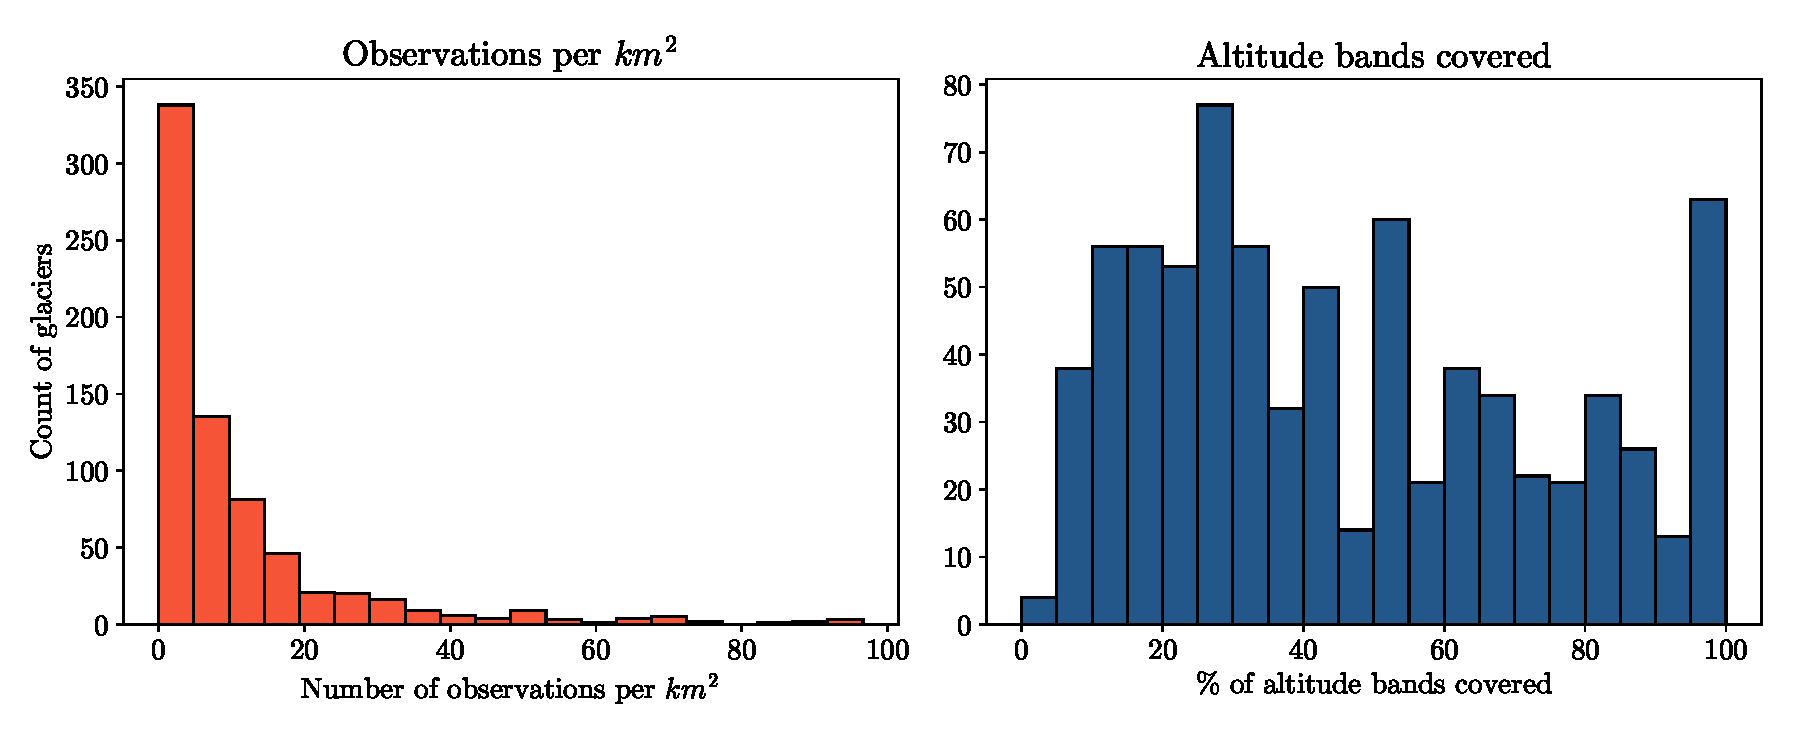
\includegraphics[width=1.\textwidth]{figures/Observations_per_skm.pdf}
	\caption{On the Left: distribution of glaciers with less than 100 observations per squared kilometer; there is a great number of glaciers with less than 20 thickness observations per squared kilometer. On the right: distribution of glaciers according to the percentage of their altitude bands covered.}
	\label{fig:glaobs}
\end{figure}

More than 91\% of all the glaciers (represented in the figure above) have less than 100 thickness measurements per squared kilometer. Almost 44\% of all the glaciers with thickness observations have less than 5 observations per squared kilometer (see Fig. \ref{fig:glaobs}).

OGGM was used to generate a gridded map of each glacier represented in the GlaThiDa. With this map one can divide each glacier in $100m$ altitude bands to check how many of those bands contain at least one thickness measurement.
Almost half of the glaciers have observations in at least half of the 100m altitude bands (see Fig. \ref{fig:glaobs}). Glaciers with few observations but well distributed over their length can be very useful for understanding glacier thickness patterns and for model validation.

\subsubsection{Survey Year}
Measurements were taken between 1977 and 2015, but most of them after 2005 (see Fig. \ref{fig:glayears}). The spread in the dates of the campaigns for taking the observations could potentially create problems when trying to compare glaciers with each other to find similar patterns, but also when using the data for model validation.
Most glacier models make in fact use of digital elevation models to setup the model run. Any digital elevation model is compiled with data available at the time of its construction. The time difference between the date of data assimilation for the digital elevation model, and the date of the survey for the thickness observation, could be in the order of several years. This would create an error when validating the model.
\begin{figure}[!tp]
	\centering		  
	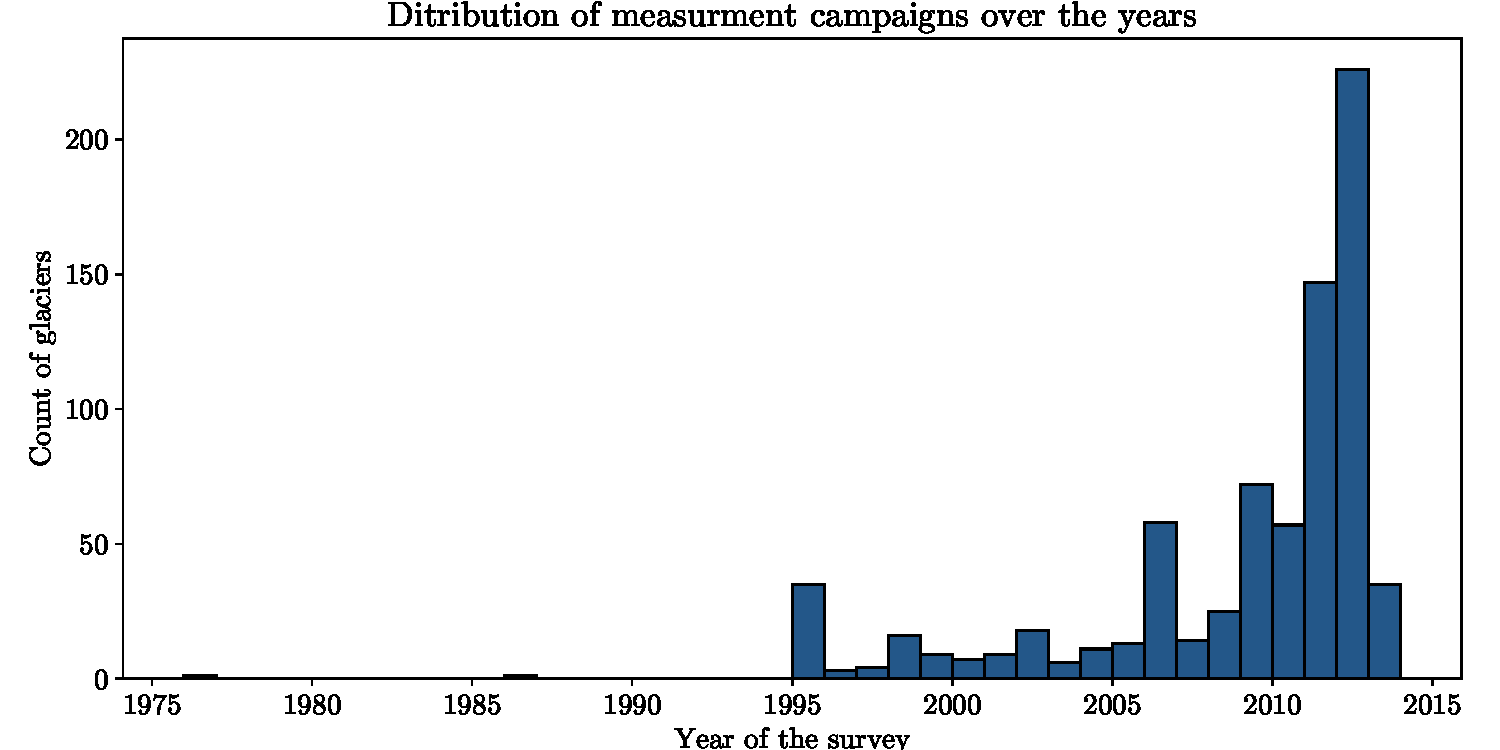
\includegraphics[width=1.\textwidth]{figures/Observations_per_year.pdf}
	\caption{Distribution of glaciers with observations in the GlaThiDa according to the year when the measurements for each glacier were taken.}
	\label{fig:glayears}
\end{figure}


\section{Choosing Features}\label{features}

\subsection{Putting together the features}
How did we get the features for training: OGGM.

\subsection{Which features did we choose}
The features we chose and why.

\section{Machine Learning Algorithms}\label{ML}
Machine learning is a mathematical method which enables computers to perform a specific task without giving it the specific instructions on how to do it. This is achieved using algorithms to build a model from data usually called the ``training data''. This data are given to the algorithm which uses an iterative process to create the final model. 

The idea behind it is to emulate the learning process of a human-being in order to make predictions about new data. If for example one wanted to teach a kid how to recognize a cat, the simpler approach would be to show it cats or pictures of them, instead of trying to explain it what are the key attributes which characterize cats. In the same way machine learning algorithm are used to make predictions without giving them instructions (explaining the key characteristics) about how to do the predictions, but rather by feeding them examples.

The branch of machine learning used in this thesis is called ``supervised learning'' which builds models learning from data which contain the input variables and the desired output value.
The machine learning algorithm is then used to find the target function $f$ which better maps input vector $X$ to an output one $Y$.
\begin{equation}
Y = f(X)
\end{equation}
The way this function is computed by the algorithm depends on the specific one chosen to achieve the desired result.

In this thesis three different machine learning algorithm have been used to train models which estimate the ice thickness of glaciers using the GlaThiDa database as the desired output ($Y$) for the ice thickness, and using digital elevation models and some basic physics assumptions as the input values ($X$), to obtain the ice thickness distribution of the glacier.

The three algorithm used are:
\begin{itemize}
	\item Linear Regression
	\item Random Forest Regression
	\item Support Vector Machine Regression (SVM)
\end{itemize}
%The way the algorithm achieves this without instructions from the programmer is with an iterative process which uses the training data to make a first prediction, compare the prediction with the the desired output value, 

\subsection{Tuning parameters}
How did we decide which parameters to use (maybe we can just leave it for the appendix)

\subsection{SVM}
Explain Support Vector Machine (do i need to write down the specific mathematics?)

\subsection{Random Forest}
Random Forest

\subsection{Linear Regression}
Linear Regression

\section{Training method}\label{training}
use sklearn train\_test\_split 20 times

\section{Scoring method}\label{scoring}
metrics to compare the goodness of models

\section{Features Importance}\label{featuresimp}
what is feature importance.

\subsection{Shuffle}
Shuffle

\subsection{partial dependence plot}
partial dependence plot 
%\subsubsection{Subsubsection}
%You can also use ``subsubsections''. However, they do not carry a separate
%heading number and they do not appear in the Table of Contents.

%\subsection{Equation}
%As an example for the \verb|equation| environment, I show the equations used in
%the numerical shallow-water model (SWM) developed by
%\citet{scha93Aag,scha93Bag}:
%% ---- equation 1:
%\begin{equation}
%\frac{D\hat{u}}{D\hat{t}}+\frac{\partial(\hat{h}+\hat{H})}
%                               {\partial\hat{x}}=0,
%\label{2equ:1}
%\end{equation}
%% ---- equation 2:
%\begin{equation}
%\frac{D\hat{v}}{D\hat{t}}+\frac{\partial(\hat{h}+\hat{H})}
%                               {\partial\hat{y}}=0,
%\label{2equ:2}
%\end{equation}
%% ---- equation 3:
%\begin{equation}
%\frac{\partial\hat{H}}{\partial\hat{t}}+\frac{\partial(\hat{u}\hat{H})}
%                                             {\partial\hat{x}}
%                                       +\frac{\partial(\hat{v}\hat{H})}
%                                             {\partial\hat{y}}
%                                                =0,
%\label{2equ:3}
%\end{equation}
%with the non-dimensional variables (henceforth generally labelled with hats)
%$\hat{u}$ and $\hat{v}$ as the two horizontal velocity components, $\hat{H}$ and
%$\hat{h}$ as fluid layer depth and terrain height, respectively,
%$\hat{Z}=\hat{h}+\hat{H}$ as fluid layer height, and $\hat{t}$ as time.
%Equations~(\ref{2equ:1})--(\ref{2equ:3}) are non-dimensionalized with the
%following scales: a typical length $L$ for the horizontal length scale, the
%initial far-upstream depth of the fluid layer $H_{\infty}$ (with $h_{\infty}=0$)
%for the vertical length scale, the phase speed of linear gravity waves
%$\sqrt{g^*H_{\infty}}$ for the velocity scale, and the time scale
%$L/\sqrt{g^*H_{\infty}}$.

\newpage
\thispagestyle{plain}


% ==== CHAPTER 3 ===============================================================
% ---- set some counters to zero:
\setcounter{equation}{0}
\setcounter{table}{0}
\setcounter{figure}{0}
% ---- include tex-file:
\chapter{Results}\label{chap3}
\thispagestyle{plain}

As mentioned in Section \ref{chap2}, three machine learning algorithms have been trained, and the resulting models used to predict glaciers ice thickness. The same procedure has been applied to all the algorithms used, in order to compare the results between the different models. 
All the algorithm have been trained and tested using the data available in the GlaThiDa data-set in the Alpine region. Only glaciers present in the GlaThiDa database belonging to region 11 of the RGI (Central Europe) have been used in the following analysis.

After training each algorithm the resulting model has been used to predict the ice volume of all the glaciers in the Alps. This is useful to compare the results of these models to those computed by \citet{Farinotti2019}.

\section{Results from Linear Regression}\label{linear}
The first model to be analyzed is the one obtained from training the linear regression algorithm. In order to assess how well a machine learning model makes predictions, a sub-sample of the data-set is usually left out from the training process (see section \ref{training}). With the left out data the score from Eq. \ref{eq:score} is computed by letting the model predict the values not used for training. This is done to make sure the model is not over-fitted. Complex machine learning algorithm in fact might be very good at predicting data inside the training sample but might perform much worse on data outside this sample (over-fitting). 
This is usually not the case with linear regression, hence in principle there is no need to only use a sub-sample of the data to train the model. The $R^2$ coefficient (the score) could be computed using the whole data-set to train the model. The linear regression algorithm however, has been trained using the same procedure used for the other algorithms, to be able to better compare the models with each other, and try to find similarities and differences.     

\subsection{Score and volume spread}\label{lr-score}

\begin{figure}[!tp]
	\centering		  
	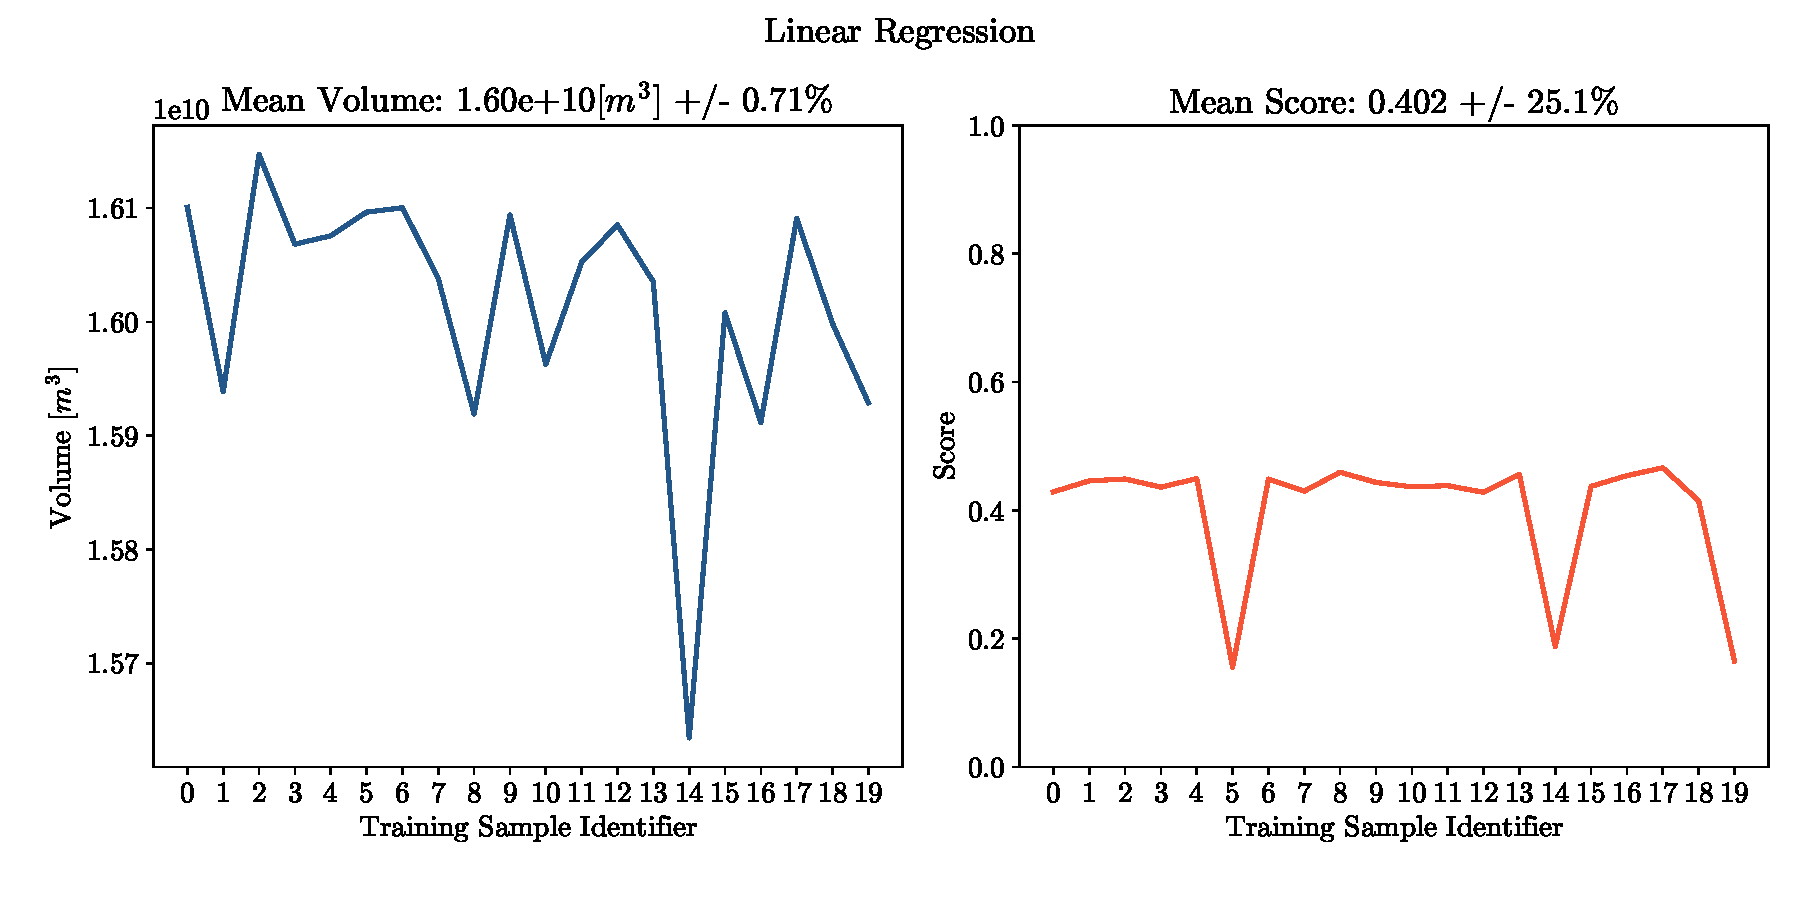
\includegraphics[width=1.\textwidth]{figures/LR_score.pdf}
	\caption{Linear Regression: Volume and score values of the model after training it with 20 different sub-sample of data. On the x-axis each number identifies a different sample of data. On the left the total volume of the alpine glaciers present in the GlaThiDa is shown. On the right the $R^2$ coefficient for values left out of the training sample.}
	\label{fig:lr-score}
\end{figure}

Figure \ref{fig:lr-score} shows the volume and score for 20 different sub-samples used to train the linear regression algorithm. Each number on the x-axis represents a different sample used for training: of all the alpine glacier observations in the GlaThiDa, 75\% of them have been used to train the model and the remaining 25\% to compute the score. 

The volume shown on the left side of Fig. \ref{fig:lr-score} has been computed on the full sample of alpine glaciers with ice thickness observations. Each value shown in the figure is obtained with a different model, derived from training it with the sub-samples. The mean volume for the 20 different sub-samples is $1.60\times 10^{10}$ $m^3$ with a relative standard deviation of 0.74\%. Sample 14 predicts the lowest of all volumes.

\begin{figure}[!tp]
	\centering		  
	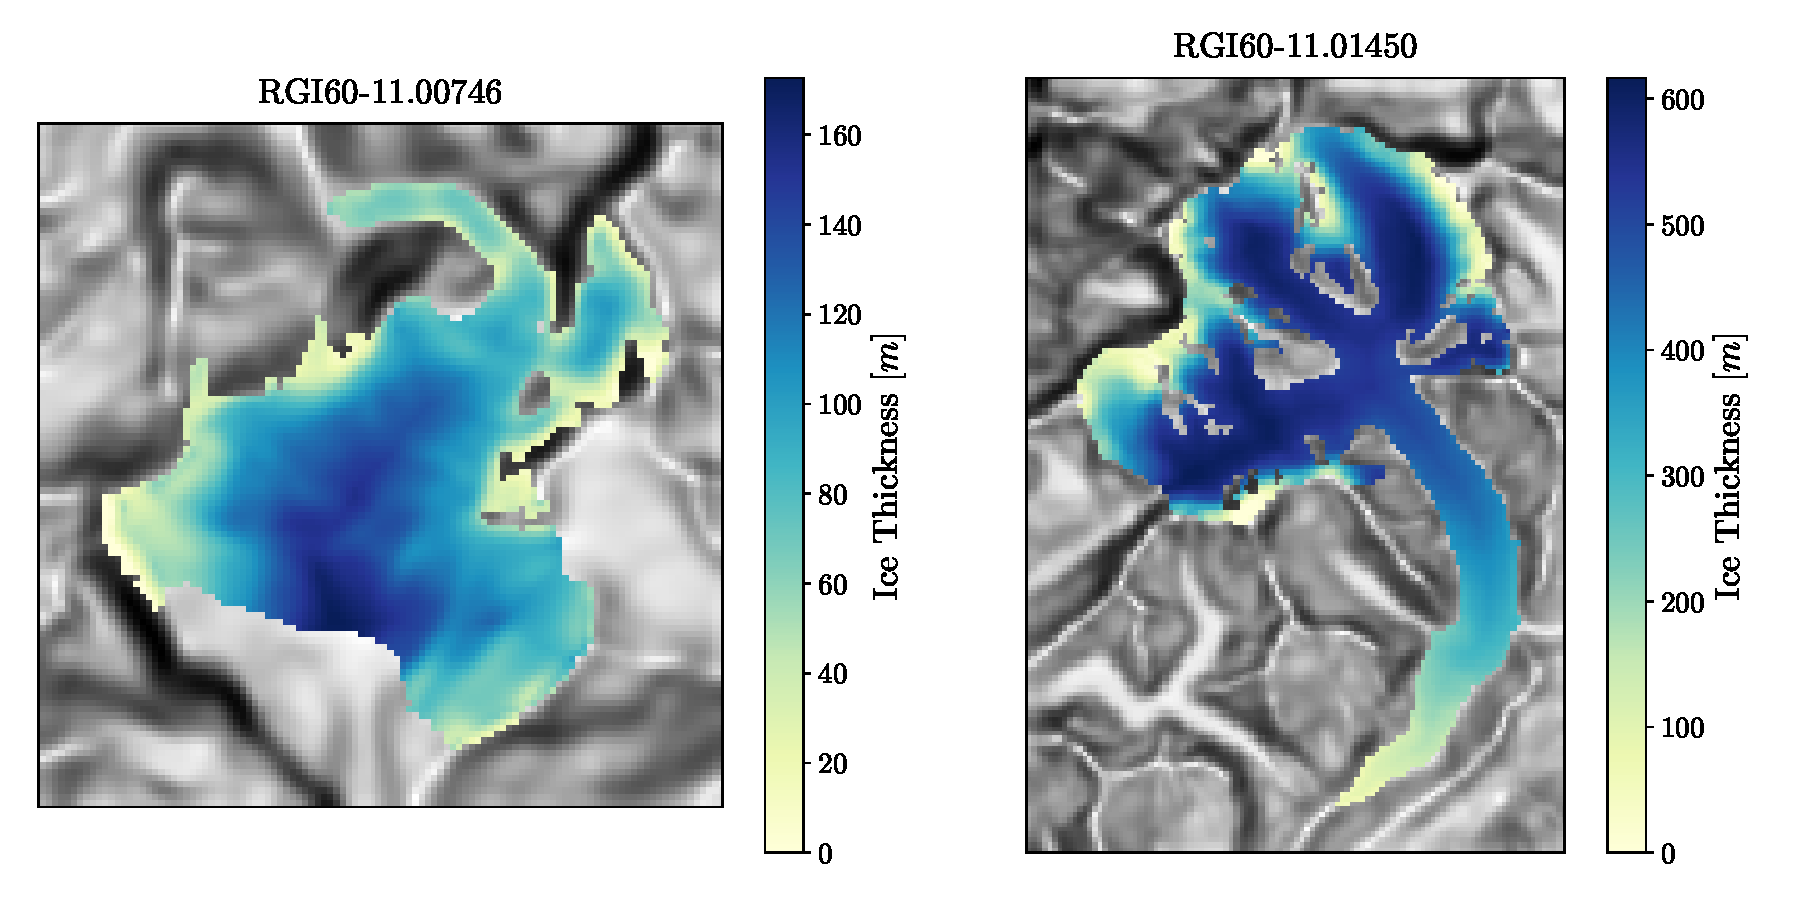
\includegraphics[width=1.\textwidth]{figures/LR_thick_map.pdf}
	\caption{Linear Regression: Ice thickness distribution for two glaciers on top of the terrain slope angle. On the left, one of the glaciers used to train the model. On the right, one of the glaciers outside those used to train the model.}
	\label{fig:lr-map}
\end{figure}

It is worth nothing that the model predicts ice thicknesses below zero for certain points. These have however been rounded to zero as a thickness below zero makes no physical sense.

The average score is 0.402 with a high 25.1\% relative standard deviation. Clearly this is due to the score dropping for sub-samples 5, 14 and 19. For most sub-samples the score is in fact above 0.4, but for those three it drops even below 0.2. Sub-sample 14 then leads to the lowest volume and a low score compared to the average.
The linear regression model trained with all the data in the data-set has score of 0.32 which  is the lowest among the three models used.

\begin{figure}[!tp]
	\centering		  
	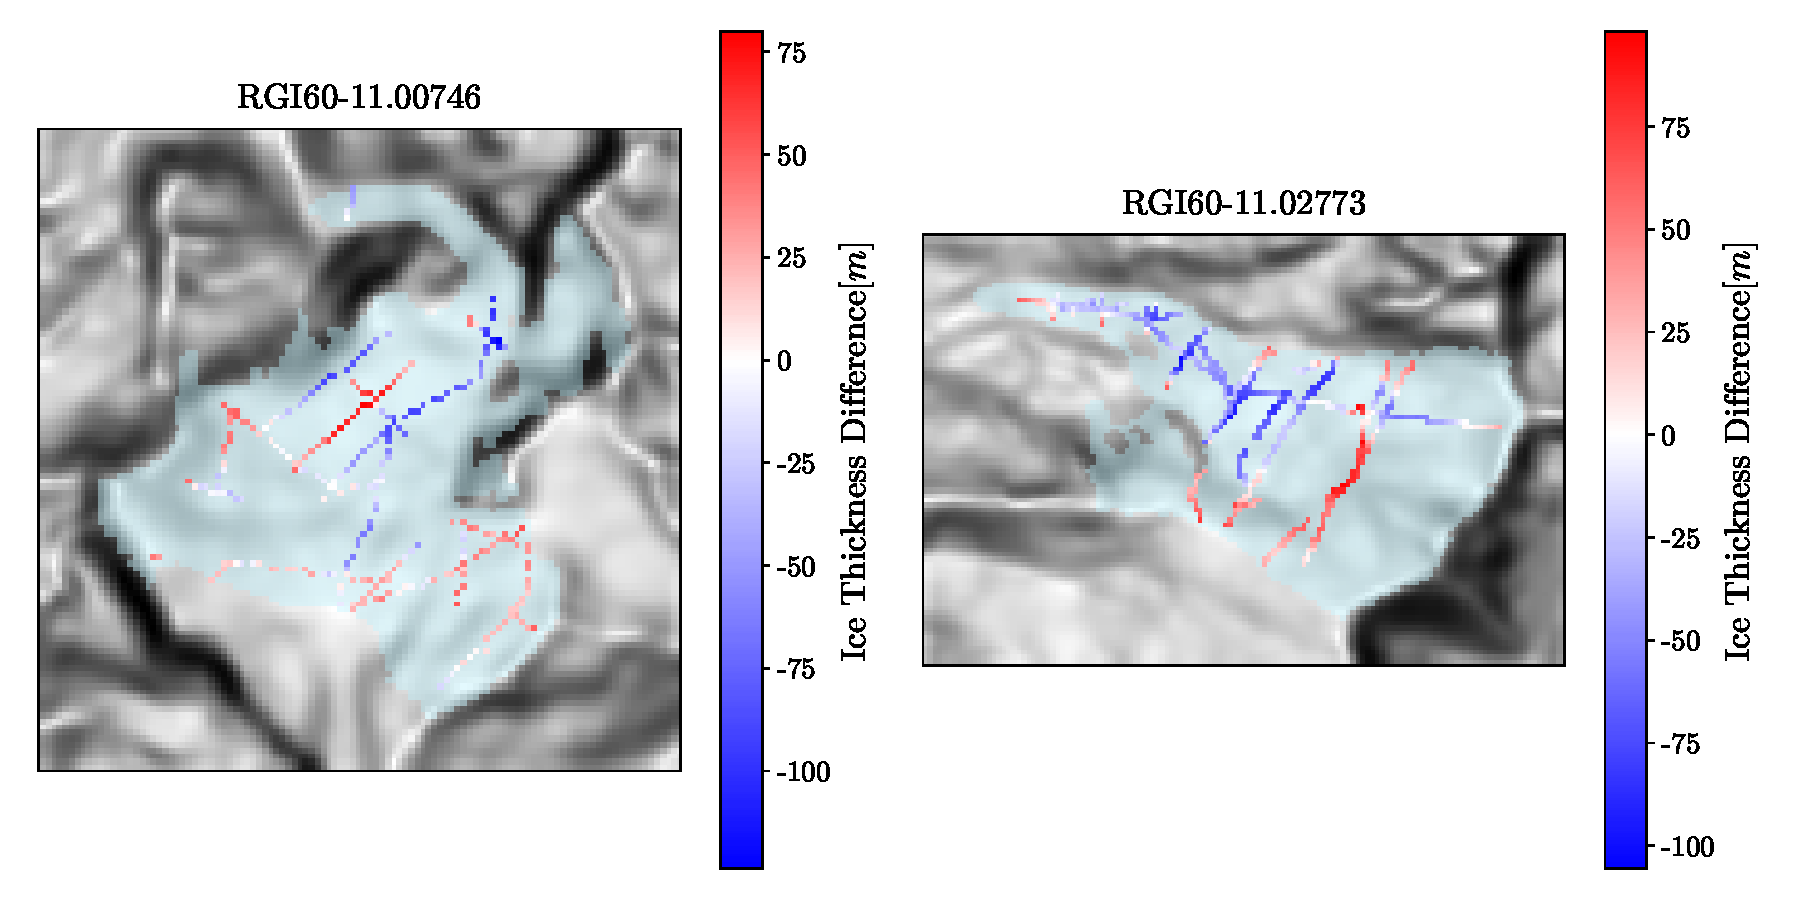
\includegraphics[width=1.\textwidth]{figures/LR_thick_diff_map.pdf}
	\caption{Linear Regression: Maps of two glaciers showing the glaciers surface and the difference between the modeled ice thickness and the  observed one.}
	\label{fig:lr-diff-map}
\end{figure}

Fig. \ref{fig:lr-map} and \ref{fig:lr-diff-map} show respectively the ice thickness distribution, and the difference in ice thickness between the observations and the model, for the linear regression. Looking at the ice thickness distribution the model seem to predict a plausible distribution. These values have been achieved by training the model on the whole sample of observations available for the alpine region.
 
The ice thickness difference from the observations for both glaciers reveals only few points to be accurately predicted by the model. Differences of of up to 100m are shown for both glaciers. For glacier RGI60-11.00746, Gepatschferner, the the model seem to do a better job at predicting the upper part of the glacier compared to the middle-bottom part. Particularly in this part it seems like for the center of the glacier the model overestimates the ice thickness while underestimating it for points lying closer to the glacier border. For glacier RGI60-11.02773 very few points seem to be predicted accurately. In particular, for the middle-bottom part of the glacier, and the central glacier flow-line, the model seem to almost always underestimate the ice thickness with values going from 25m to up to 100m lower than the observed ice thickness. In the top part of the glacier the highest positive differences are registered.

After training the linear regression model with all the available observations for the alpine glaciers, their total volume estimated by the linear regression is $1.40 \times 10^{11}m^3$, which is 9.8\% larger than the volume predicted by \citet{Farinotti2019}.


\subsection{Features Importance}  

It is interesting to look into which of the variables used to train the model influence the outcome of the prediction the most.

A very easy way to do so for a linear regression model, is just to analyze the weights $\bm{\beta}$ (see Eq. \ref{eq:linear}), which the model assigned to each feature in order to make predictions. These are shown in Table \ref{tb:lr-coef}.
The higher the absolute values of the coefficients, the more the variable will influence the outcome of the model. Looking at these coefficients, the slope angle is the feature which is more relevant to the outcome of the model, followed by the linear mass balance. In particular the slope influences the prediction almost 3 times more than the altitude and over 2.5 times more than the distance from the border. This means that a doubling of the slope angle of the glacier surface, will result in an ice thickness change 3 times larger than the change predicted by a doubling of the altitude. It is worth noting that the slope angle has a negative sign, meaning that lower slope angles correspond to higher ice thicknesses in accordance with the literature about glaciers ice flow \cite[P. 298]{cuffey2010physics}.

\begin{table}
	\centering
	\caption{Linear Regressions: Coefficients for the linear regression model: higher absolute values mean that the feature have a higher influence on the model predictions}
	\begin{tabular}{|c|c|c|c|}
		\hline 
		Slope Angle&Mass Balance&Distance From Border&Altitude \\
		\hline
		-19.7&12.7&7.7&-6.6 \\
		\hline
	\end{tabular}
	\label{tb:lr-coef}
\end{table}

The results form the coefficients analysis of the linear model, could be enough to have a complete picture about the variables influencing the output the most. An analysis showing the tools used for the other models is shown anyway, in order to have comparable results between the models, and to understand how these tools compare with the method of analyzing the magnitude of the linear model coefficients. 

Figure \ref{fig:lr-heatmap} shows the coefficients deriving from the permutation analysis explained in section \ref{permutation}. This looks at changes in the score of the model, when the feature values for a single feature are shuffled randomly. If the score doesn't change, compared to the one achieved by the model with the correct order of the features values, it would mean that the feature is less relevant in making predictions. The higher the permutation coefficient value, the more relevant is the feature in making predictions. Figure \ref{fig:lr-heatmap} shows that using this method the slope angle is the feature which most influences the outcome of the prediction, which is in accordance with the values of the model coefficients in table \ref{tb:lr-coef}. Also for the other features the permutation shows the same result already found with the model coefficients. Interestingly for sub-sample 5, 14 and 19, there is a significant drop in the permutation coefficient for all of the features. These were also the sub samples with the lowest score, registered in the score analysis for the linear regression model.

\begin{figure}[!tp]
	\centering		  
	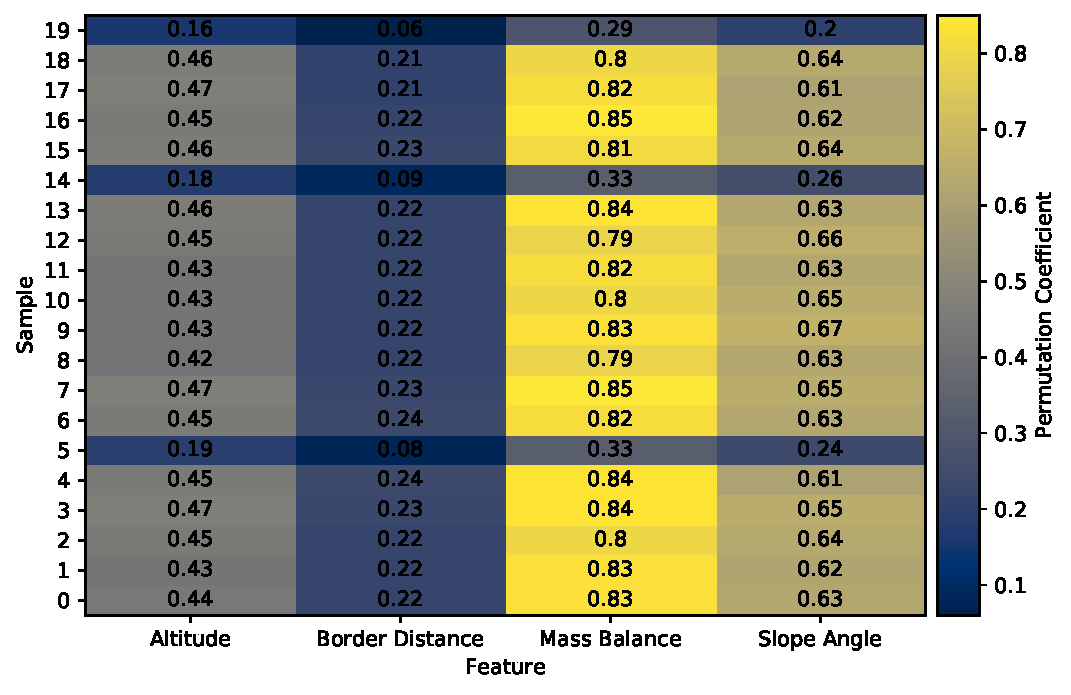
\includegraphics[width=1.\textwidth]{figures/LR_heatmap.pdf}
	\caption{Linear Regression permutation coefficients heatmap: each row in the figure represents a sub-sample of the data used for training the algorithm. Each column represents the permutation coefficient value for the considered feature.}
	\label{fig:lr-heatmap}
\end{figure}

Finally Fig. \ref{fig:lr-pdp} shows the change in thickness value for changes in values of the features. Features are scaled according to Eq. \ref{eq:scale}, hence the values on the x-axis of the figure do not represent the original input values, but the scaled ones used to train the model. Having scaled features helps reading this chart as features could have very different ranges and scales (for example altitudes ranging between  $2000m$ and almost $5000m$, compared to slope angles ranging from $0$ to $\frac{\pi}{2}$). Each line represents ice thickness changes when all other variables are kept constant. This provides for a visual comparison between the influence which each feature has on the prediction. For the linear regression case each line is a of course a straight line, but this will not be the case for the other models. Looking at the chart the same conclusions as for both the linear coefficient magnitude, and the permutation importance can be drawn.

\begin{figure}[!tp]
	\centering		  
	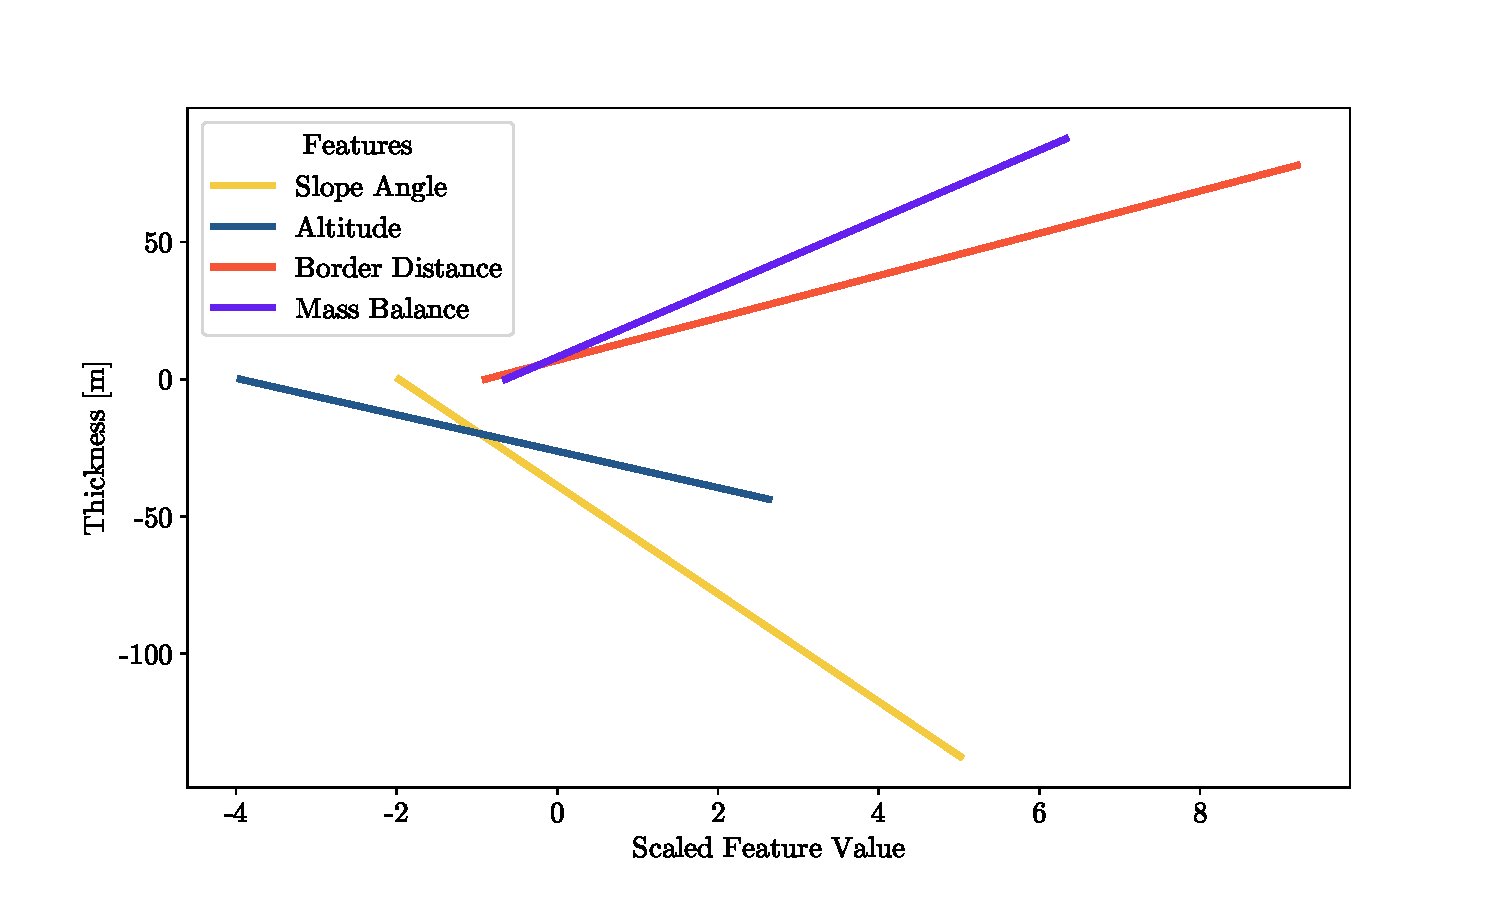
\includegraphics[width=1.\textwidth]{figures/LR_pdp.pdf}
	\caption{Linear Regression partial dependence plots: representation of the change in Ice Thickness compared to the change in the value of the features. Features values are scaled according to Eq. \ref{eq:scale}}
	\label{fig:lr-pdp}
\end{figure}

\section{Random Forest Regression}\label{rfr}
The same process of using different sub-samples to train the algorithm and test its performance used in the linear regression case, has been used for the random forest algorithm. This is particularly important for random forests because they are very prone to over-fitting. Especially the parameters determining the maximum tree depth, and the one determining the minimum number of samples required to split the tree, are those which had to be carefully adjusted in order to maintain a good balance between the model performances, and its inability to generalize for samples not used to train it. The maximum tree depth parameter has been tuned in order for all the nodes to be expanded, until all the samples at the node would have the same label, or until the minimum sample necessary for the tree to split would be reached. The minimum sample required for the tree to split has been set to 5\% of the number of samples present in the training data-set.  

\subsection{Score and volume spread}\label{rfr-score}

\begin{figure}[!tp]
	\centering		  
	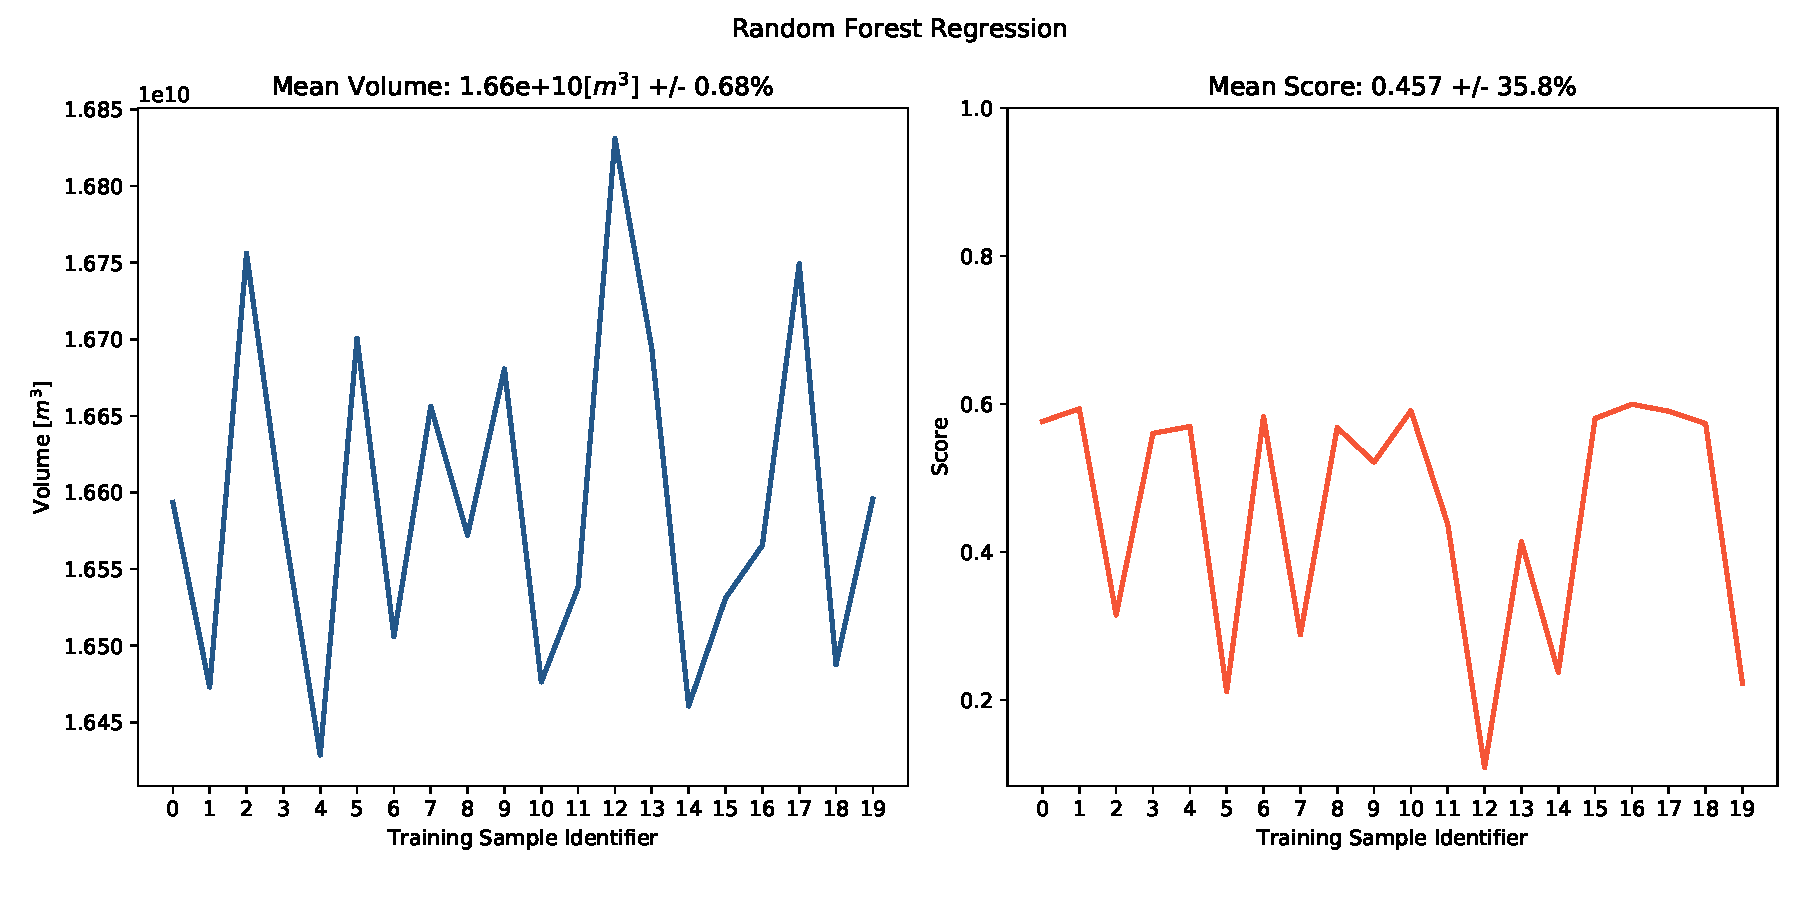
\includegraphics[width=1.\textwidth]{figures/RFR_score.pdf}
	\caption{Random Forest Regression: Volume and score values of the model after training it with 20 different sub-sample of data. On the x-axis each number identifies a different sample of data. On the left the total volume of the alpine glaciers present in the GlaThiDa. On the right the $R^2$ coefficient for values left out of the training sample.}
	\label{fig:rfr-score}
\end{figure}

Figure \ref{fig:rfr-score} shows the volume and score for 20 different sub-samples used to the random forest regression. 

It must be reminded that as the name of the algorithm suggests, part of its training process is random, due to the random processes used to create the different trees of the forest (see section \ref{random-forest}). This means that training the model again could produce slightly different results then the ones shown in Fig. \ref{fig:rfr-score}.

The score shown seems to be dependent on the sample used for training. This could mean that the model has been over-fitted, but it's also a common characteristic of random forest algorithms (\citet{RandomForest2018}). For some samples the score is around 0.6 but it gets as low as almost 0 for sample 12. As for the linear regression case low scores are registered for samples 5, 14 and 19 but also for samples 8, and 12. 
The model trained with all the data available from GlaThiDa reached a score 0.57, which is the highest of all the models tested.


\begin{figure}[!tp]
	\centering		  
	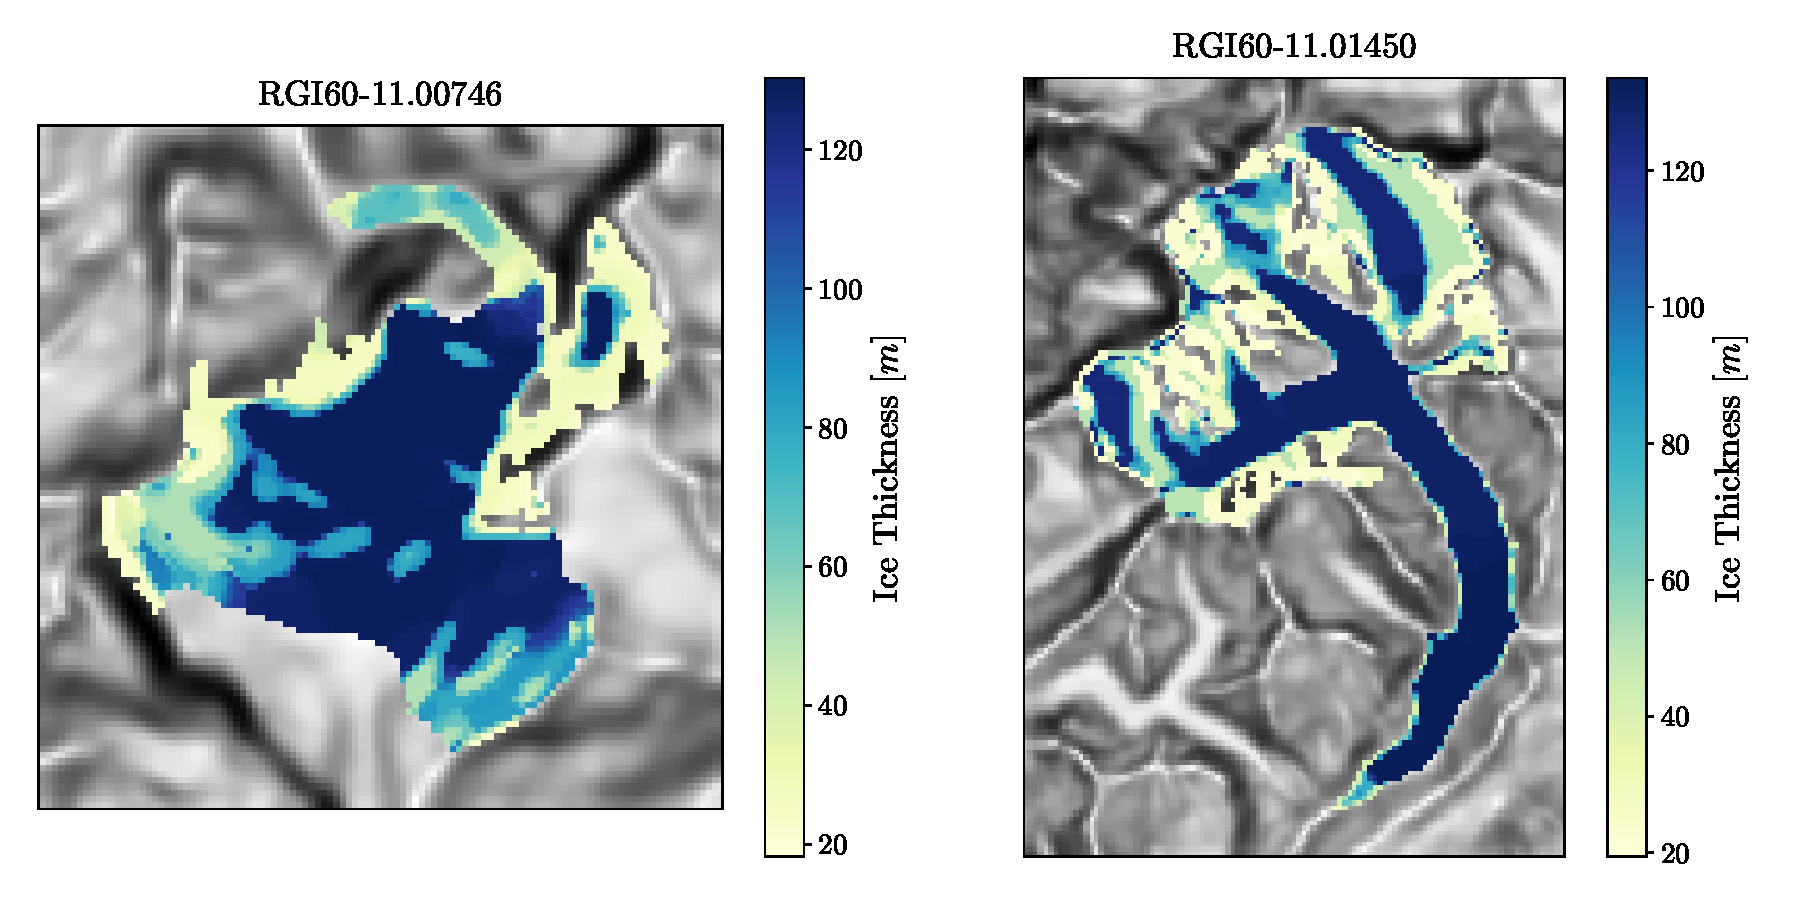
\includegraphics[width=1.\textwidth]{figures/RFR_thick_map.pdf}
	\caption{Random Forest Regression: Ice thickness distribution for two glaciers on top of the terrain slope angle. On the left, one of the glaciers used to train the model. On the right, one of the glaciers outside those used to train the model.}
	\label{fig:rfr-map}
\end{figure}

\begin{figure}[!tp]
	\centering		  
	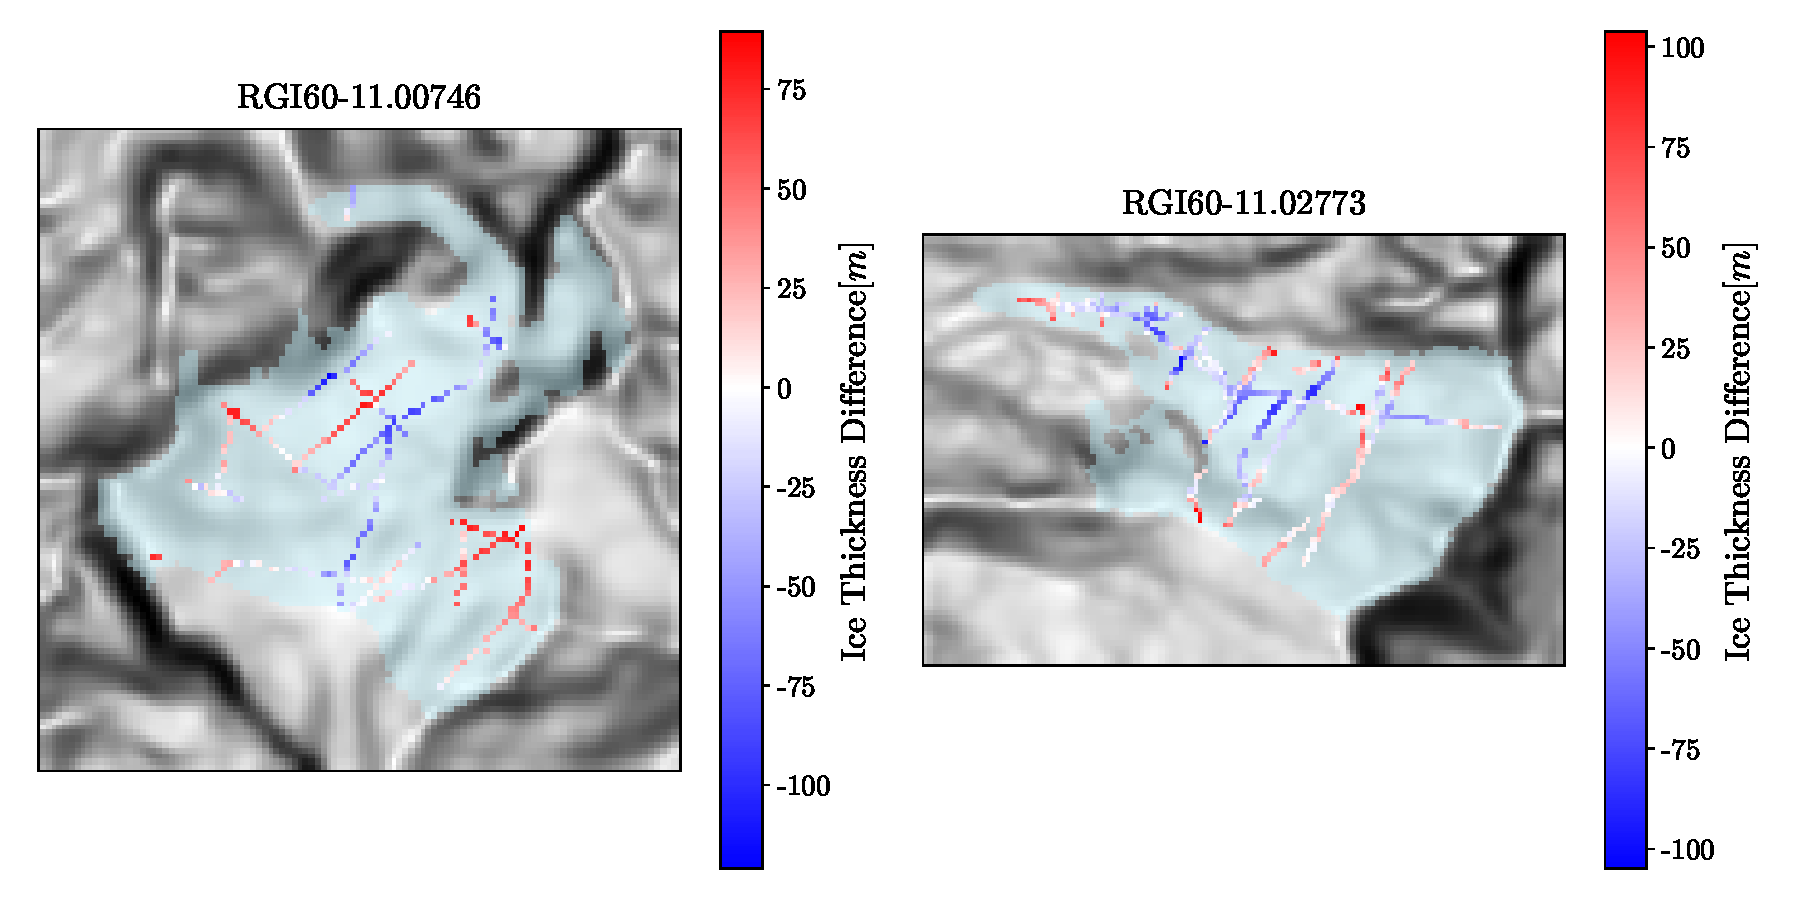
\includegraphics[width=1.\textwidth]{figures/RFR_thick_diff_map.pdf}
	\caption{Random Forest Regression: Maps of two glaciers showing the glaciers surface and the difference between the modeled ice thickness and the observed one.}
	\label{fig:rfr-diff-map}
\end{figure}

Contrary to the score values, the volume spread is not that high. The model seems to fail to correctly predict specific ice thickness, and its score is influenced by the sample chosen for training. This does not however seem to influence the total volume predicted for the glaciers for which this volume has been computed.

In Fig. \ref{fig:rfr-map} the ice thickness distribution predicted by the model trained using all the available observations for two different glaciers is shown. The ice thickness distribution seems to be distributed in a rather discontinuous way, with large areas of the glaciers having relatively high but constant ice thickness values. It is also notable that the extreme values for ice thickness in both glaciers are the same. All this is to be expected for the random forest regression, as the values predicted at each leaf by the model are the mean of the ice thickness values for the samples which reached that leaf. This both implies that abrupt changes in ice thickness are to be expected and that the model is not able to predict values higher than the maximum ice thickness value reached in the training data-set.

Fig. \ref{fig:rfr-diff-map} shows the difference in ice thickness between the model prediction and the observations. For both glaciers differences up to 100m are shown. For glacier RGI60-11.00746 ice thicknesses higher than the ones observed are visible in the middle-bottom part of the glacier towards its center and lower ones towards the border. This is similar to what already shown for the linear regression model. Higher predictions are very pronounced also in the top part of the glacier. For glacier RGI60-11.02773 the model predictions still show high differences with the observations, but the largest differences  seem to be less frequent compared to RGI60-11.02773. For this glacier the model predicts lower values than observed more frequently than higher ones. In general it seems to do a better job predicting this glacier ice thickness compared to the former one.

The total volume for the alpine glaciers computed with the random forest regression model trained with all the available observations is $9.96 \times 10^{10}m^3$, which is 22.1\% lower than the volume predicted by \citet{Farinotti2019}.

\subsection{Features Importance}\label{rfr-features}

As for the linear regression model, random forest regression allows for a direct way of computing how influential each feature is at making predictions. This is computed as the total decrease in node variance, weighted by the proportion of samples reaching the node, averaged over all trees in the ensemble (see section \ref{random-forest}). This is a very convenient way of determining the importance of the features, but it has been found biased in some cases (\citet{RandomFBias2007}). For this reason performing a permutation importance test on the model, can help to confirm the results obtained from the variance reduction method. 

Figure \ref{fig:rfr-heatmap} shows the coefficients deriving from the permutation analysis on the left, and the feature importance deriving from the variance reduction on the right. Both are calculated using the models trained with the different training samples already used for the score analysis. The feature importance heatmap on the right predicts the slope angle to be the most important of the features. In fact it computes it to be on average 1.6 times more important than the mass balance in making predictions. Altitude and distance from the border seem to be of almost no relevance in making predictions for both the methods used. However the permutation importance points at the mass balance as the most important feature. The difference in the coefficients of the mass balance and the slope angle computed with the permutation importance analysis, isn't as pronounced as the difference for the same coefficients calculated with the variance reduction method. The values for the permutation importance of mass balance and slope angle are in fact very similar.

\begin{figure}[!tp]
	\centering		  
	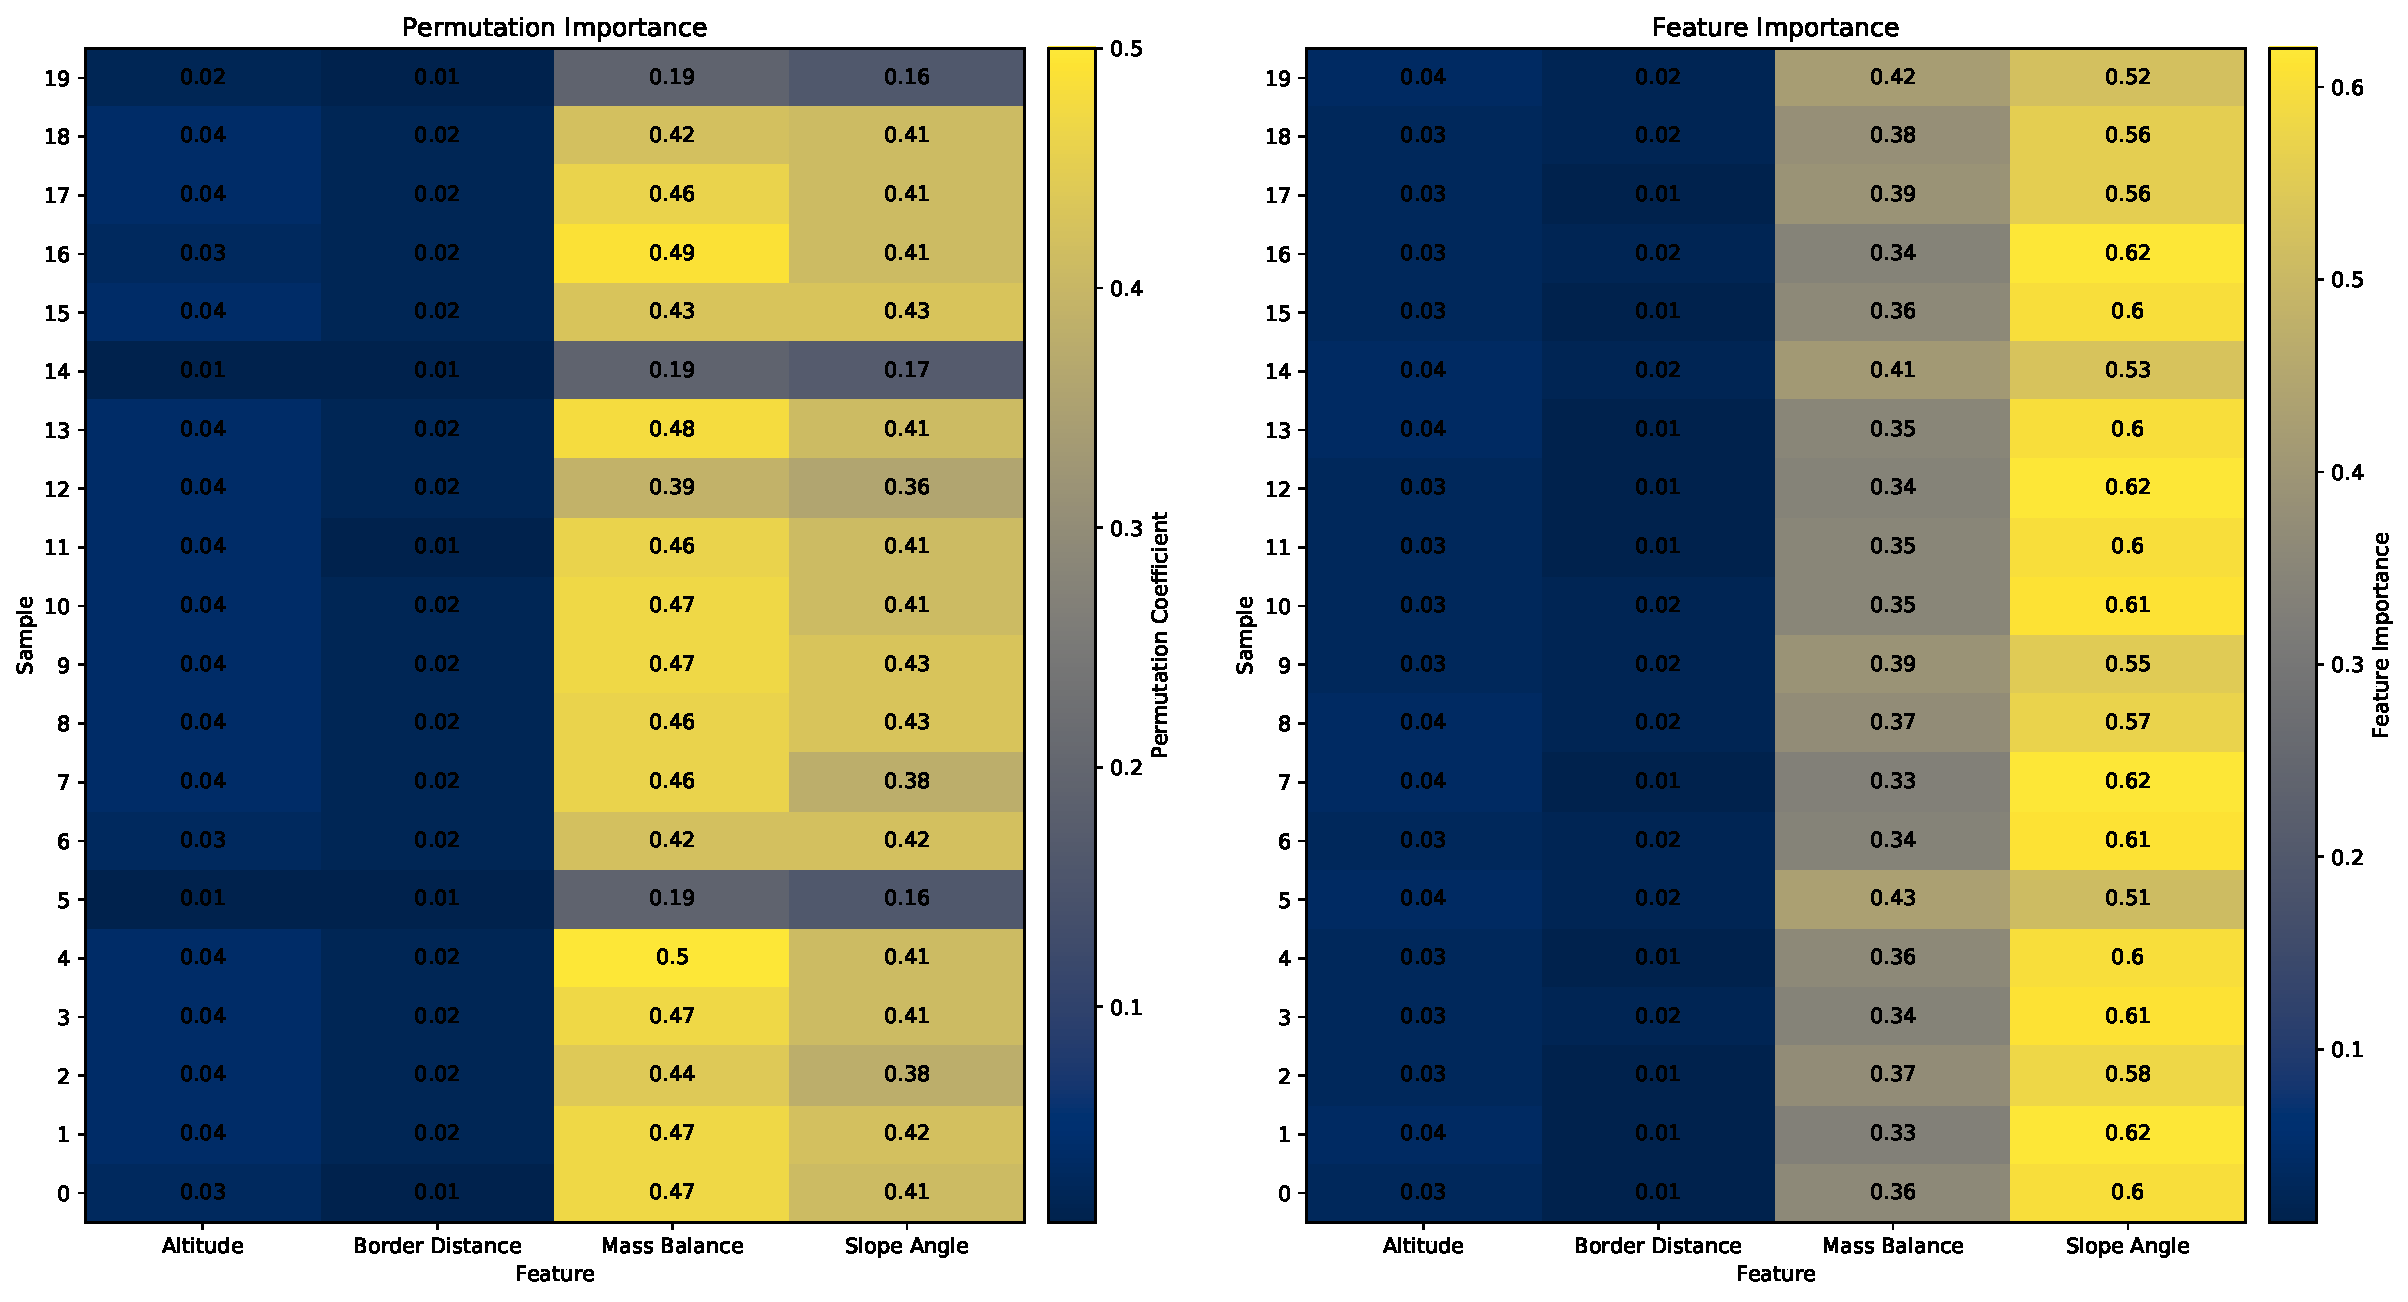
\includegraphics[width=1.\textwidth]{figures/RFR_heatmap.pdf}
	\caption{Random Forest Regression feature importance heatmaps: On the left the permutation coefficient; on the right the feature importance from the variance reduction method. Each row in the figure represents a sub-sample of the data used to train the algorithm. Each column represents respectively the permutation coefficient (left) or the variance reduction (right) value for the considered feature.}
	\label{fig:rfr-heatmap}
\end{figure}

Fig. \ref{fig:rfr-pdp} shows the change in thickness value for changes in values of the features. Once again, feature values are scaled according to Eq. \ref{eq:scale}. Immediately one sees that the change in ice thickness is not linearly dependent from the change in feature value. All the lines don't look continuous and present clear steps marking the change in ice thickness. This is partly due to the possible abrupt change in feature value, but it is mostly a natural effect of the sharp splits happening in the node of a decision tree.  The mass balance has a change in its slope going from increasing to decreasing around 0 and then increasing again around 1.8. The slope line has a sudden pick and changes from decreasing to increasing just below 0. The altitude also is slightly non monotonic between -1 and 0 while the border distance is always monotone. 
\begin{figure}[!tp]
	\centering		  
	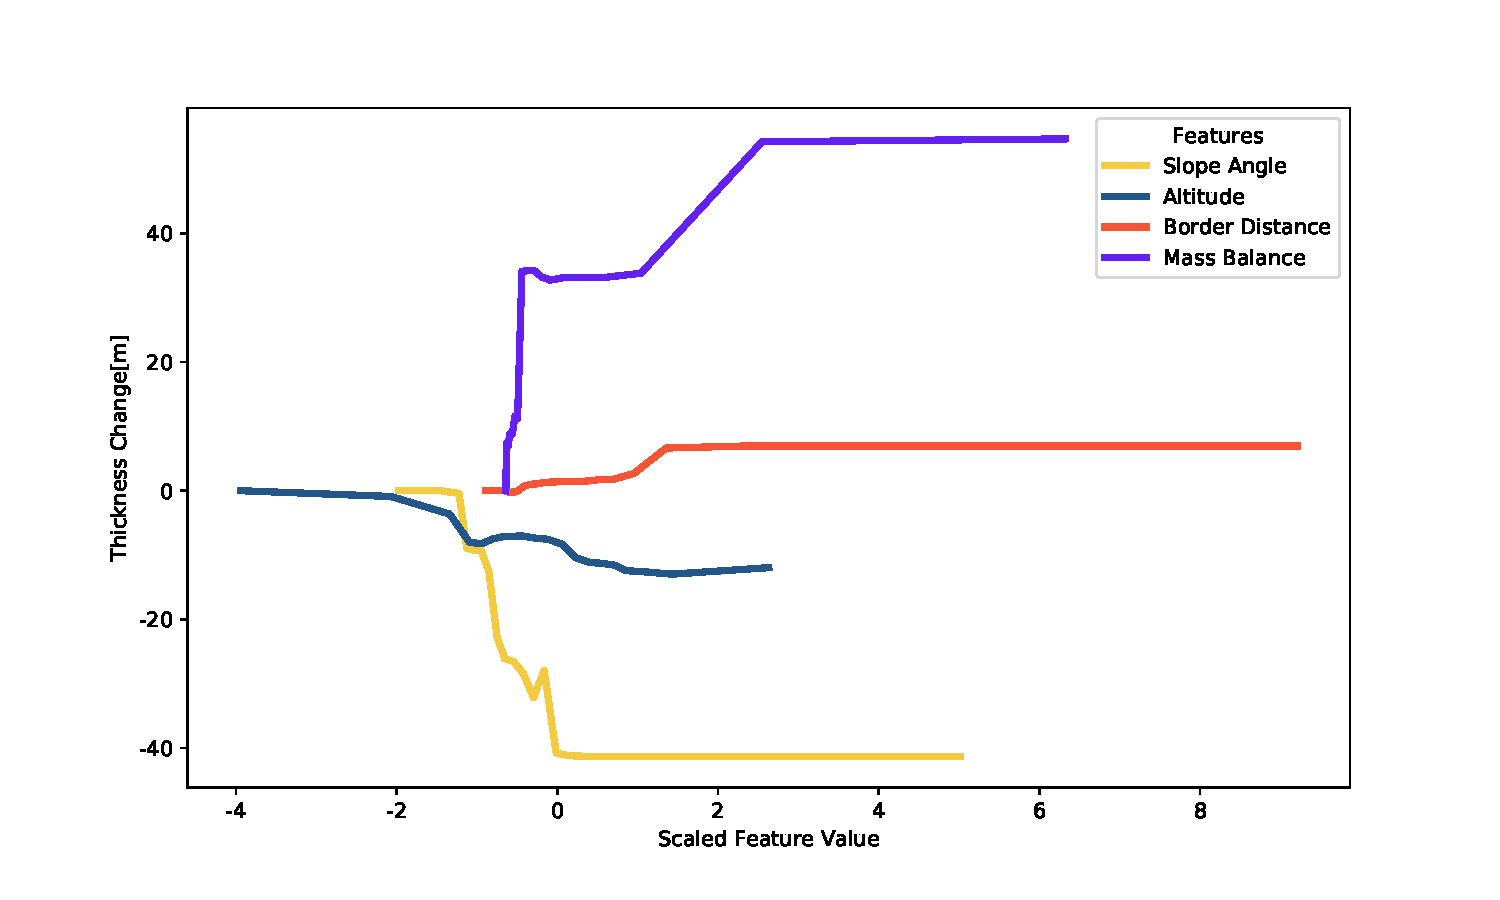
\includegraphics[width=1.\textwidth]{figures/RFR_pdp.pdf}
	\caption{Random Forest Regression partial dependence plots: representation of the change in Ice Thickness compared to the change in the value of the features. Features values are scaled according to Eq. \ref{eq:scale}}
	\label{fig:rfr-pdp}
\end{figure}

Fig. \ref{fig:rfr-pdp} also is in accordance with the feature importance analysis showed in the heatmaps of Fig. \ref{fig:rfr-heatmap} as the altitude and border distance seem to lead to very small changes in the ice thickness prediction. Looking at the partial dependence plots, it also seems like the slope leads to a change in ice thickness up until the scaled value reaches 0 (around $18^{\circ}$ angle). After this value the ice thickness prediction doesn't change. The maximum range of ice thickness change achieved by the slope angle is $40m$. For the mass balance there seem to be a change in ice thickness prediction throughout the whole range of its values up until scaled values just below 3. The steepest changes happen for values below 0. Its range in changes in ice thickness is almost $60m$ which is higher than the changes attributed to the slope angle.


\section{Support Vector Regression}\label{svr}
Support Vector Regression is the last model for which the results are presented here. The training process for this algorithm is notably slower compared to the linear regression and the random forest. However it is the model which reached the highest average score between the ones used. 

\subsection{Score and volume spread}\label{svr-score}

\begin{figure}[!tp]
	\centering		  
	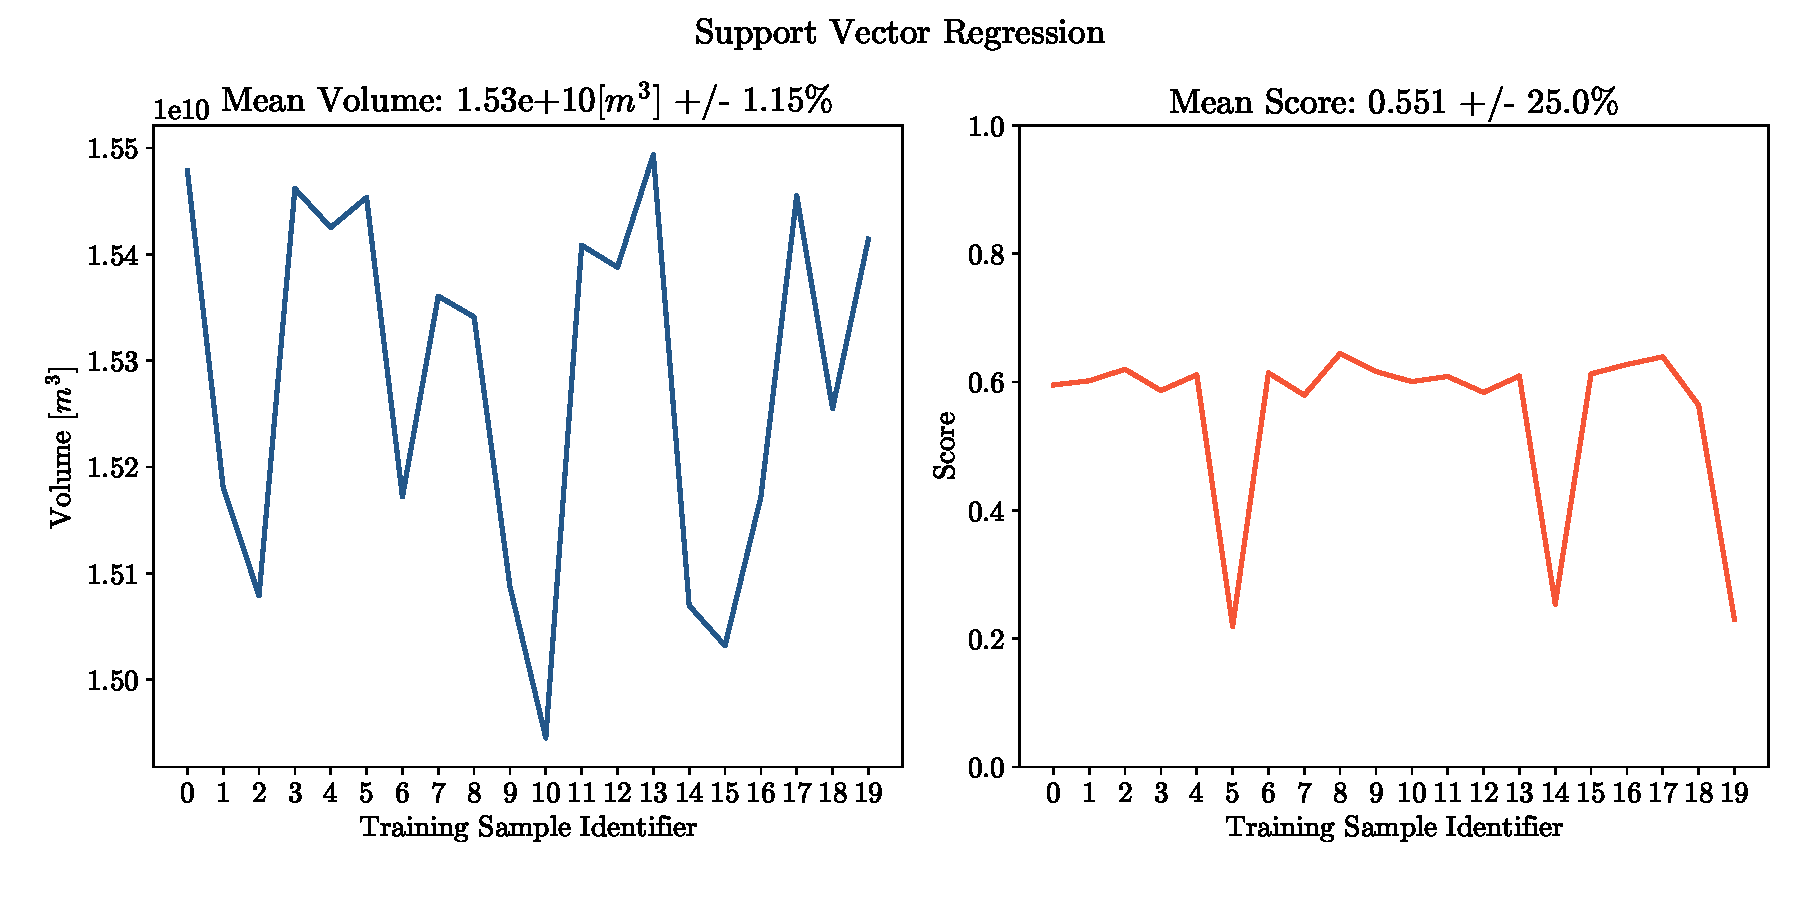
\includegraphics[width=1.\textwidth]{figures/SVR_score.pdf}
	\caption{Support Vector Regression: Volume and score values of the model after training it with 20 different sub-sample of data. On the x-axis each number identifies a different sample of data. On the left: the total volume of the alpine glaciers present in the GlaThiDa. On the right: the $R^2$ coefficient for values left out of the training sample.}
	\label{fig:svr-score}
\end{figure}

Fig. \ref{svr-score} shows on the left the volume spread for the alpine glaciers with ice thickness observations, and on the right the score of the model as defined in \ref{eq:score}. Each of the different values represents a model trained with a different sub-sample of data, the same sub-samples already used for the linear regression and random forest regression analysis.

The score shows a very similar pattern compared to the one shown in the linear regression model (see Fig. \ref{fig:lr-score}). Samples 5, 14 and 19 present a drop in the score achieved, exactly as already shown for the linear regression case. The average score however is higher reaching 0.55 on average and it is around 0.6 for most of the sub-samples used to train the model.
The value of the score for the model trained with all the data available from GlaThiDa is 0.45, which means that less than 50\% of the ice thickness variance is explained by the model. 

The volume spread on the left of the figure shows a dispersion around 1.15\% and an average total volume of $1.53 \times 10^{10}m^3$. This is the lowest of all the models considered so far. 
Looking at Fig. \ref{fig:svr-map}, the ice thickness distribution for the glacier RGI60-11.01450 immediately looks strange. The ice thickness for most of the glacier seem to be in the order of 75$m$ with much higher values only reached in the very bottom part of it. It seems that the model is actually predicting a constant ice thickness for most of the glacier. This is of course not a desirable result as ice thicknesses are presumed to change throughout the surface of the glacier. The same behavior is not visible in the left glacier which shows different ice thicknesses uniformly distributed all over the glacier surface. Notice that the left glacier is one used to train the model, while the right one isn't.

The total volume of ice for the alpine glaciers predicted by the support vector machine is $9.58 \times 10^{10}m^3$, which is the lowest of all the models and 25.1\% lower than the volume predicted by \citet{Farinotti2019} with their ensemble model.

\begin{figure}[!tp]
	\centering		  
	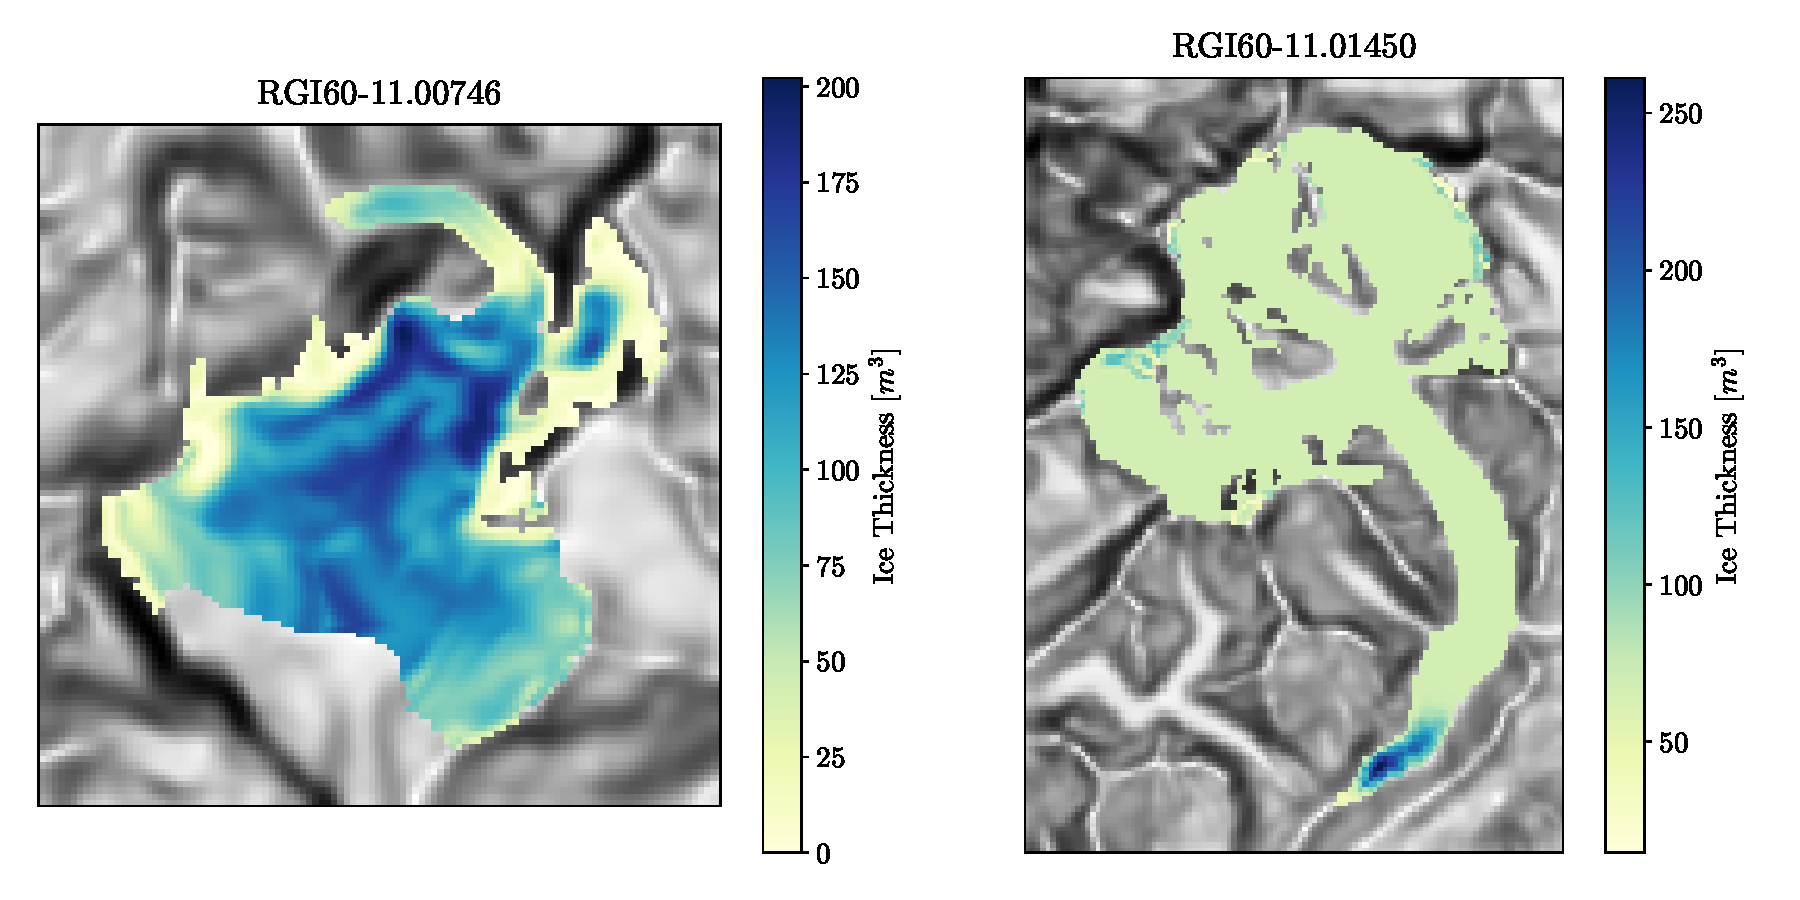
\includegraphics[width=1.\textwidth]{figures/SVR_thick_map.pdf}
	\caption{Support Vector Regression: Ice thickness distribution for two glaciers on top of the terrain slope angle. On the left one of the glaciers used to train the model. On the right one of the glaciers outside those used to train the model.}
	\label{fig:svr-map}
\end{figure}

\subsection{Features Importance}\label{svr-features}
Unlike linear and random forest regression, support vector regression doesn't have a simple way of computing the influence each feature has in making a prediction when using a non-linear kernel to transform the features. In order to analyze which features are the most important, one needs to recur to indirect methods such as the permutation importance.

\begin{figure}[!tp]
	\centering		  
	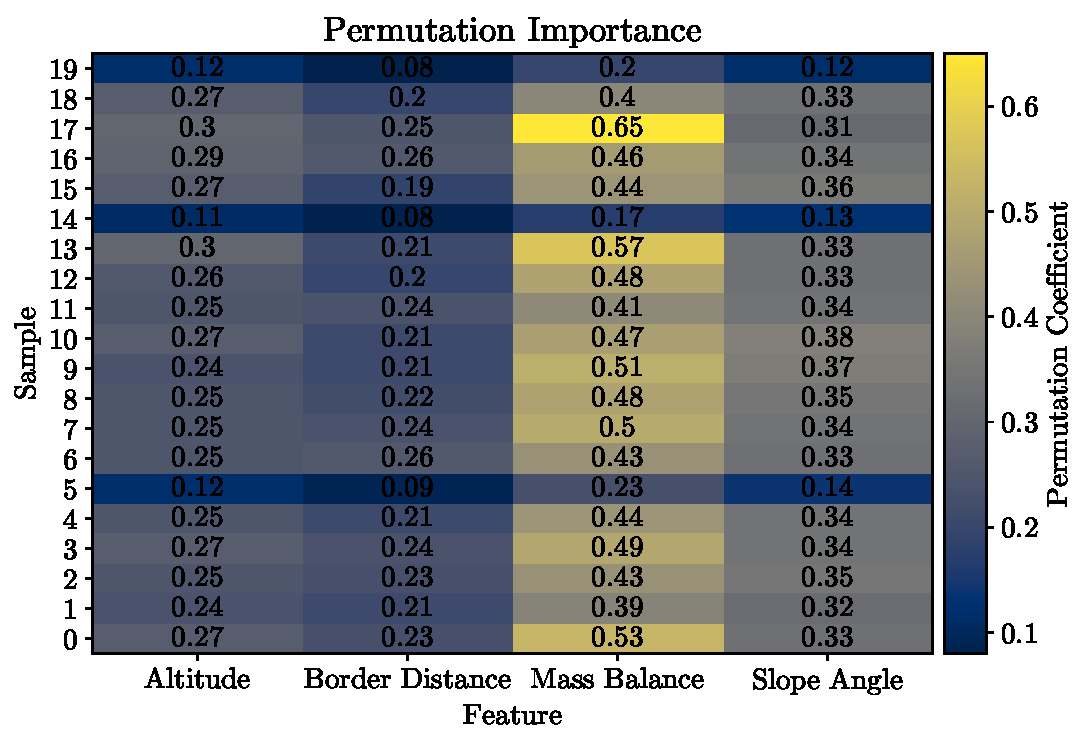
\includegraphics[width=0.8\textwidth]{figures/SVR_heatmap.pdf}
	\caption{Support Vector Regression feature importance heatmap: each row in the figure represents a sub-sample of the data used to train the algorithm. Each column represents the permutation coefficient value for the considered feature.}
	\label{fig:svr-heatmap}
\end{figure}

In Figure \ref{fig:svr-heatmap} the coefficients for the permutation importance (section \ref{permutation}) for all the models trained with the 20 different sub-samples of the data are shown. Once again the sub-samples with the lowest score registered (see Fig. \ref{fig:svr-score}), sub-samples 5, 14 and 19 are in general the ones displaying a lower value of permutation importance, showing a dark blue line throughout the whole heatmap. Apart from those sub-samples, the linear mass balance above the point is the feature with the highest permutation importance even though values vary from 0.65 to 0.39. The second highest permutation importance values are those of the slope angle. In general then the most important features for the support vector regression model are the same as those of the random forest regression model. However the permutation coefficients of altitude and distance from the border are also comparable to those of the slope angle and they are also very close to each other, with the altitude seeming to play a bigger role compare to the border distance. All the features in general seem to play a role in the model final prediction. 

To complete the analysis of how the features influence the prediction of the support vector regression, Fig. \ref{fig:svr-pdp} shows the change in thickness value depending on changes in feature value. Again, the non-linear relation between the two is evident in this chart.  None of the curve is monotone and for each feature the ice thickness seems to increase or decrease depending on the value of the specific feature. Mass balance and slope angle drive the largest ice thickness changes looking at the range of those changes reached by those features curves. For feature values between 2 and 1 however the rate of change in ice thickness is similar between the altitude and slope angle, meaning that both these features compete in determining the ice thickness for those range of values. The same thing happens for values between around -0.5 and around 1.8 for the border distance and the linear mass balance, where again the two seem to compete in determining the predicted ice thickness.
\begin{figure}[!tp]
	\centering		  
	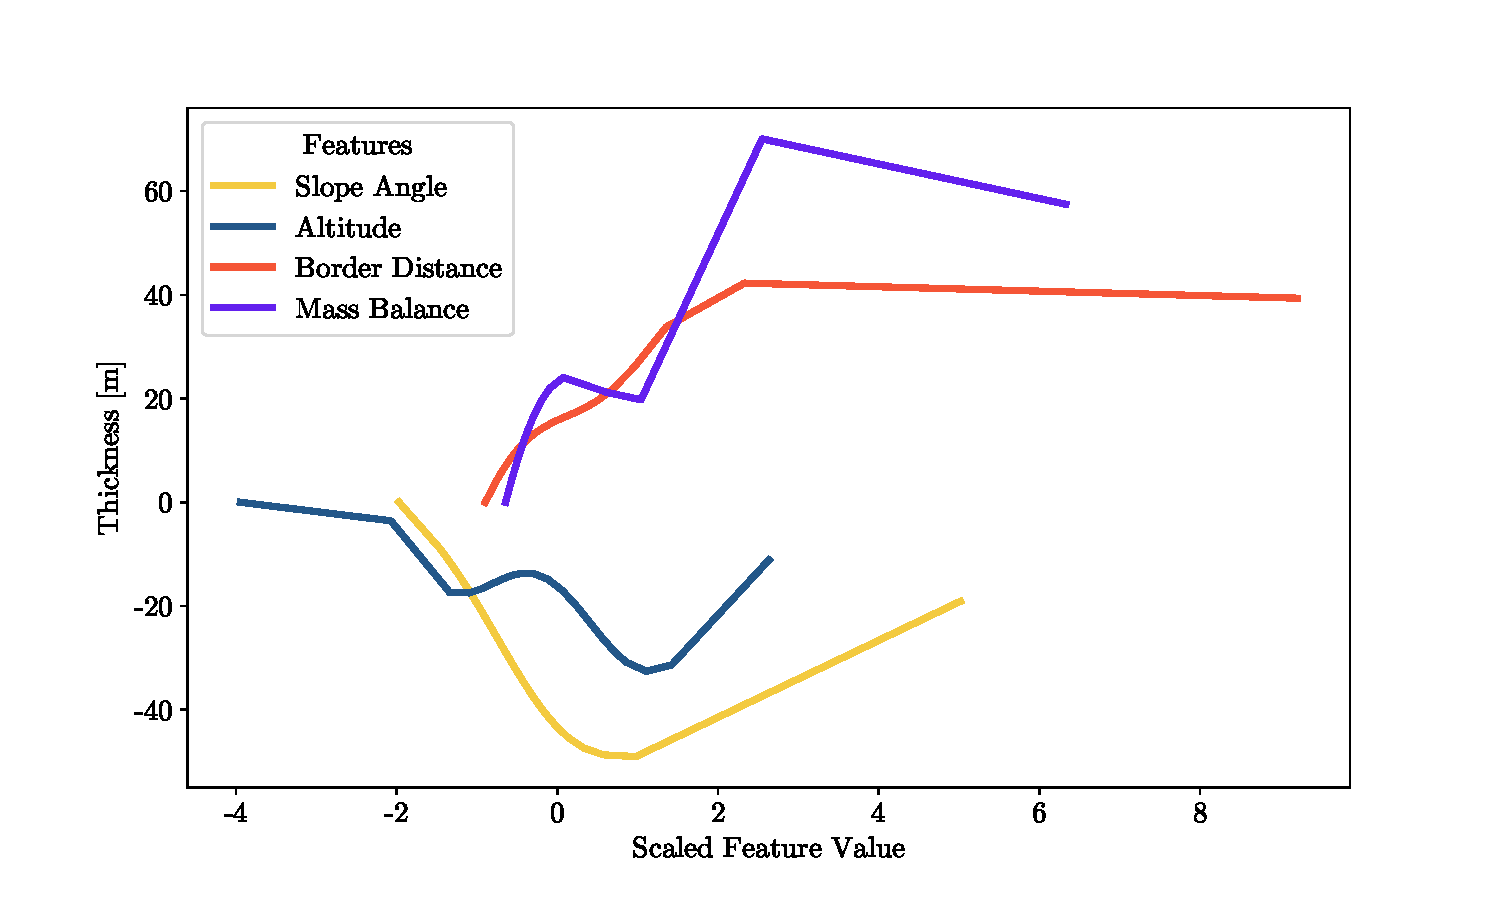
\includegraphics[width=1.\textwidth]{figures/SVR_pdp.pdf}
	\caption{Support Vector Regression partial dependence plots: representation of the change in Ice Thickness compared to the change in the value of the features. Features values are scaled according to Eq. \ref{eq:scale}}
	\label{fig:svr-pdp}
\end{figure}

This also seems to be in accordance with the analysis obtained with the permutation importance coefficients (see Fig. \ref{fig:svr-heatmap}). All features in fact seem to have some relevance in predicting the ice thickness at least for some of their value ranges. Mass balance and slope angle however seem to be more relevant throughout all their value ranges and also lead to a larger change in ice thickness, when looking at the minimum and maximum ice thickness change reached by their extreme values. 


% ==== SECTION 1 ===============================================================
%\section{Some Important Things to Know}\label{3sec:1}
%
%It is important to differentiate between \emph{facts} and \emph{interpretations}
%and between \emph{your contributions} and \emph{those of others}! Facts and
%your contributions are part of this chapter. Interpretations and contributions
%of others should be rather part of the chapter Discussion.
%
%
%\subsection{Experimental Parts in the Chapter Results}
%Experimental details should only appear in the chapter Results to the
%extent necessary to ensure comprehension. Painstaking descriptions of
%instruments, analysis procedures, field conditions, etc., should be part of the
%chapter Methodology. However, absolutely necessary is information that shows
%the \emph{reliability} of the findings and the \emph{robustness} of an
%innovation (e.g., a new analysis technique).
%
%
%\subsection{Numerical Results or so-called Data}
%Results are more than simply numbers! They are tiny but unique
%\emph{messages}. Data should not only be made ``visible'' (e.g., in
%figures, such as in Fig.~\ref{fig:1}) but should also be made
%\emph{articulate}.
%
%
%\subsection{Order of Presentation}
%Use chapters and (sub)sections to separate, e.g., various topics,
%questions, and problems, or to separate measurements from calculations. 
%Arrange information in a consistent way, e.g., from simple to complex, from
%small to large (or vice versa in terms of scales: e.g., from
%synoptic-scale to micro-scale), from \emph{most important} (central) to
%\emph{least important} (peripheral). Arrange the material in order to maximize
%impact rather than sticking to a strict chronological order. Try to tell a story
%that consists of a beginning, followed by a gradual unfolding, and a
%``happy end''.
%
%
%\subsection{Cross-References}
%You can always refer to other parts of your thesis like in the following
%example: See chapter \ref{chap2} or section \ref{1sec:3} or
%Fig.~\ref{fig:1} or Table~\ref{tab:1} or equation~(\ref{2equ:1}).
%
%
%\section{Figure}\label{3sec:2}
%Figure \ref{fig:1} shows an example for an EPS figure with two panels. The
%topography of the Wipp Valley and Inn Valley is shown in Fig.~\ref{fig:1a}.
%Figure~\ref{fig:1b} shows the time series of potential temperature at two
%stations. In order to refer to a certain range of figure panels write, e.g.,
%Fig.~\ref{fig:1a}--\subref{fig:1b}.
%
%
%\begin{figure}[!tp]
%\centering
%\figuretopcapfalse
%\subfigure[][]{
%  \label{fig:1a}  
%  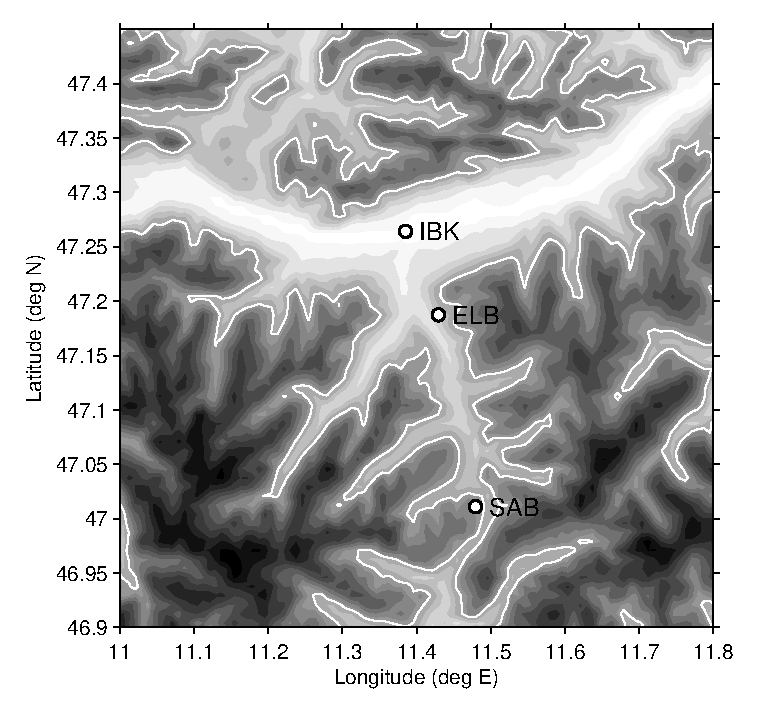
\includegraphics[width=0.48\textwidth]{figure_topo.eps}
%}
%\subfigure[][]{
%  \label{fig:1b}
%  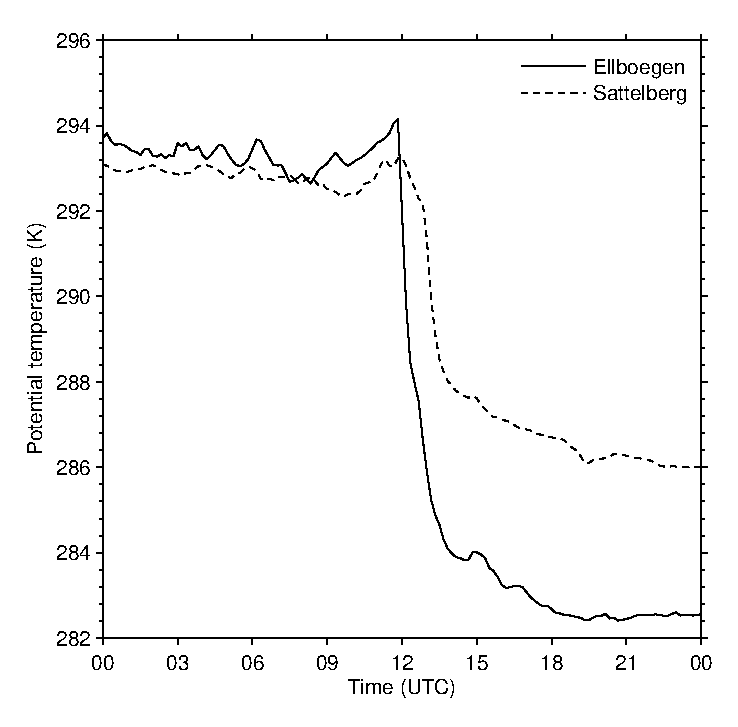
\includegraphics[width=0.47\textwidth]{figure_theta.eps}
%}
%\caption{(\subref{fig:1a}) Topographic map of the target area: Gray shaded
%elevations contours with increments of 200~m starting at 400~m~MSL and a white
%elevation contour line at 1600~m MSL. (\subref{fig:1b}) Time series of potential
%temperature (K) at Ellboegen (solid line) and Sattelberg (dashed line) from 00
%UTC 06 November to 00 UTC 07 November 1999. Labels in (\subref{fig:1a}) mark the
%location of Innsbruck (IBK), Ellboegen (ELB), and Sattelberg
%(SAB).}\label{fig:1}
%\end{figure}
%
%
%This template uses the \texttt{subfigure} environment with the option
%\texttt{FIGTOPCAP} to place the subfigure labels (\subref{fig:1a}) and
%(\subref{fig:1b}) at the top of the figure. However, since we want to have the
%caption at the bottom of figure, use \verb|\figuretopcapfalse|
%before the first \verb|\subfigure| command within the \texttt{figure}
%environment, otherwise the figure number produced by \verb|\ref| is wrong.
%
%
%\section{Table}
%Table \ref{tab:1} is an example for a table that consists of several
%rows and columns. Here, the \texttt{tabular} environment is used inside the
%\texttt{table} environment.
%
%
%\begin{table}[!htb]
%\centering
%\begin{footnotesize}
%\renewcommand{\tabcolsep}{4pt}
%\begin{tabular}{l p{3.5cm} l l l}
%\hline
%\hline
%Parameter & Code & Description & Units & Code\\
%\hline
%$g$ & \verb|$g$| & acceleration due to gravity&
%  m~s$^{-2}$ & \verb|m~s$^{-2}$| \\
%$T_d$ & \verb|$T_d$| & dew point temperature & $^{\circ}$C & 
%  \verb|$^{\circ}$C| \\
%$\mathbf{v} \cdot \nabla T$ & \verb|$\mathbf{v} \cdot| \verb| \nabla T$| &
%  temperature advection & K~s$^{-1}$ & \verb|K~s$^{-1}$| \\
%$\vec{v} \cdot \nabla T$ & \verb|$\vec{v} \cdot| \verb| \nabla T$| & 
%  temperature advection & K~s$^{-1}$ & \verb|K~s$^{-1}$| \\
%$\frac{\partial p}{\partial t}$ & \verb|$\frac{\partial p}|
%  \verb| {\partial t}$| & local pressure tendency & Pa~s$^{-1}$ &
%  \verb|Pa~s$^{-1}$| \\
%$p_0 \cos (kx - \omega t)$ & \verb|$p_0 \cos (kx| \verb| - \omega t)$| &
% wave expression & Pa & Pa \\
%\hline
%\end{tabular}
%\end{footnotesize}
%\caption{Some meteorological and mathematical parameters and expressions.}
%\label{tab:1}
%\end{table}
%
%
%\section{Figure and Table Captions}
%
%Figure and table captions \emph{must} contain all necessary information to
%understand the \emph{content} of the figure and table, without the need of
%additional text. Only in case of very complicated figures or tables, the caption
%may end with a remark such as ``See text for further explanation''. The
%\emph{interpretation} of the table or figure is not part of the caption, but
%should be given in the main text. In order to avoid repetitions, the phrase
%``As in Fig. xx, but for \dots'' is often used. Necessary information provided
%in the caption is a description of
%\begin{itemize}
%\item shown parameters together with units,
%\item date and time,
%\item contour intervals,
%\item location,
%\item line styles and markers,
%\item and others.
%\end{itemize}
%A list of figures and a list of tables at the beginning of the thesis (before
%chapter 1) is optional.
%
%
%
%\section{Title}
%
%The title of your science thesis should be kept as short as possible. It should
%represent an extremely compact summary of the thesis. The title should provide a
%clear and complete description of the topic and should contain many keywords
%(``what?'', ``how?'' and possibly ``why?''). The main title should not contain
%more than 10 words. An optional subtitle may be used if necessary (all together
%not more than 25 words). Important words and terms should be placed at the
%beginning of the title. Avoid unspecific expressions such as
%\begin{itemize}
%\item[] Investigation of ...
%\item[] Experiments on ...
%\item[] Results of ...
%\item[] Attempts to ...
%\end{itemize}
%Rather use expressions such as
%\begin{itemize}
%\item[] Influence of ... on ...
%\item[] Generation of ... with ...
%\item[] Dependence of ... upon ...
%\item[] Optimization of ... upon ...
%\end{itemize}
%Avoid technical abbreviations or acronyms and special symbols such as IR
%for infrared or $\theta$ for potential temperature.
%
%
%\section{Abbreviations and Symbols}
%Abbreviations (e.g., ECMWF) and symbols (e.g., $\vec{v}_g$) have to be
%defined, i.e. explained, at the place where the \emph{first} appear in the text.
%For example: The model was initialized with the operational analysis of the
%European Centre for Medium-Range Weather Forecasts (ECMWF). From the ECMWF
%fields of geopotential height we derive the geostrophic wind vector
%$\vec{v}_g$. The change of $\vec{v}_g$ with pressure $p$ reveals the thermal
%wind equation.
%
%A list of abbreviations and a list of symbols at the beginning of the thesis
%(before chapter 1) is optional.
%
%
%\section{Parameters and Units}
%
%Use italic letters for scalar quantities (e.g., $R$ and $g$), bold upright
%letters or arrows for vector quantities (e.g., $\mathbf{v}_g$ or $\vec{v}_g$)
%and sans-serif letters for tensors (e.g., $\mathsf{T}$). All this parameters
%should be written in mathematical mode (\verb|$ ... $|). Units should be
%written with normal upright letters (e.g., m~s$^{-1}$). Use spacing between
%numbers and individual units (e.g., $\phi=100$~W~m$^{-2}$). Less or no spacing
%is used between numbers and units in case of percent and degrees (e.g.,
%10\% and 5$^{\circ}$C). See also Table~\ref{tab:1} for further examples.
%
%
%\section{Footnotes}
%Do not use footnotes in an extensive way. Footnotes distract the reader from the
%main body of the document. Do not use footnotes for referring to literature,
%rather use the author-year citation system together with a bibliography (list
%of references) at the end of the thesis.
\newpage
\thispagestyle{plain}


% ==== DISCUSSION ==============================================================
% ---- set some counters to zero:
\setcounter{equation}{0}
\setcounter{table}{0}
\setcounter{figure}{0}
% ---- include tex-file:
\chapter{Discussion}\label{disc}
\thispagestyle{plain}
In this chapter a deeper analysis of the results from chapter \ref{chap3} are presented in order to try to understand the behavior of the models and compare their performances. A comparison of the results obtained with the models used in this thesis with the model presented by \cite{Farinotti2019} will also be conducted, as it is interesting to compare statistical based models as those deriving from machine learning algorithms, with the physical based one from  The third ITMIX.

\section{Machine learning models performances}\label{MLcomp}

\begin{figure}[p]
	\centering		  
	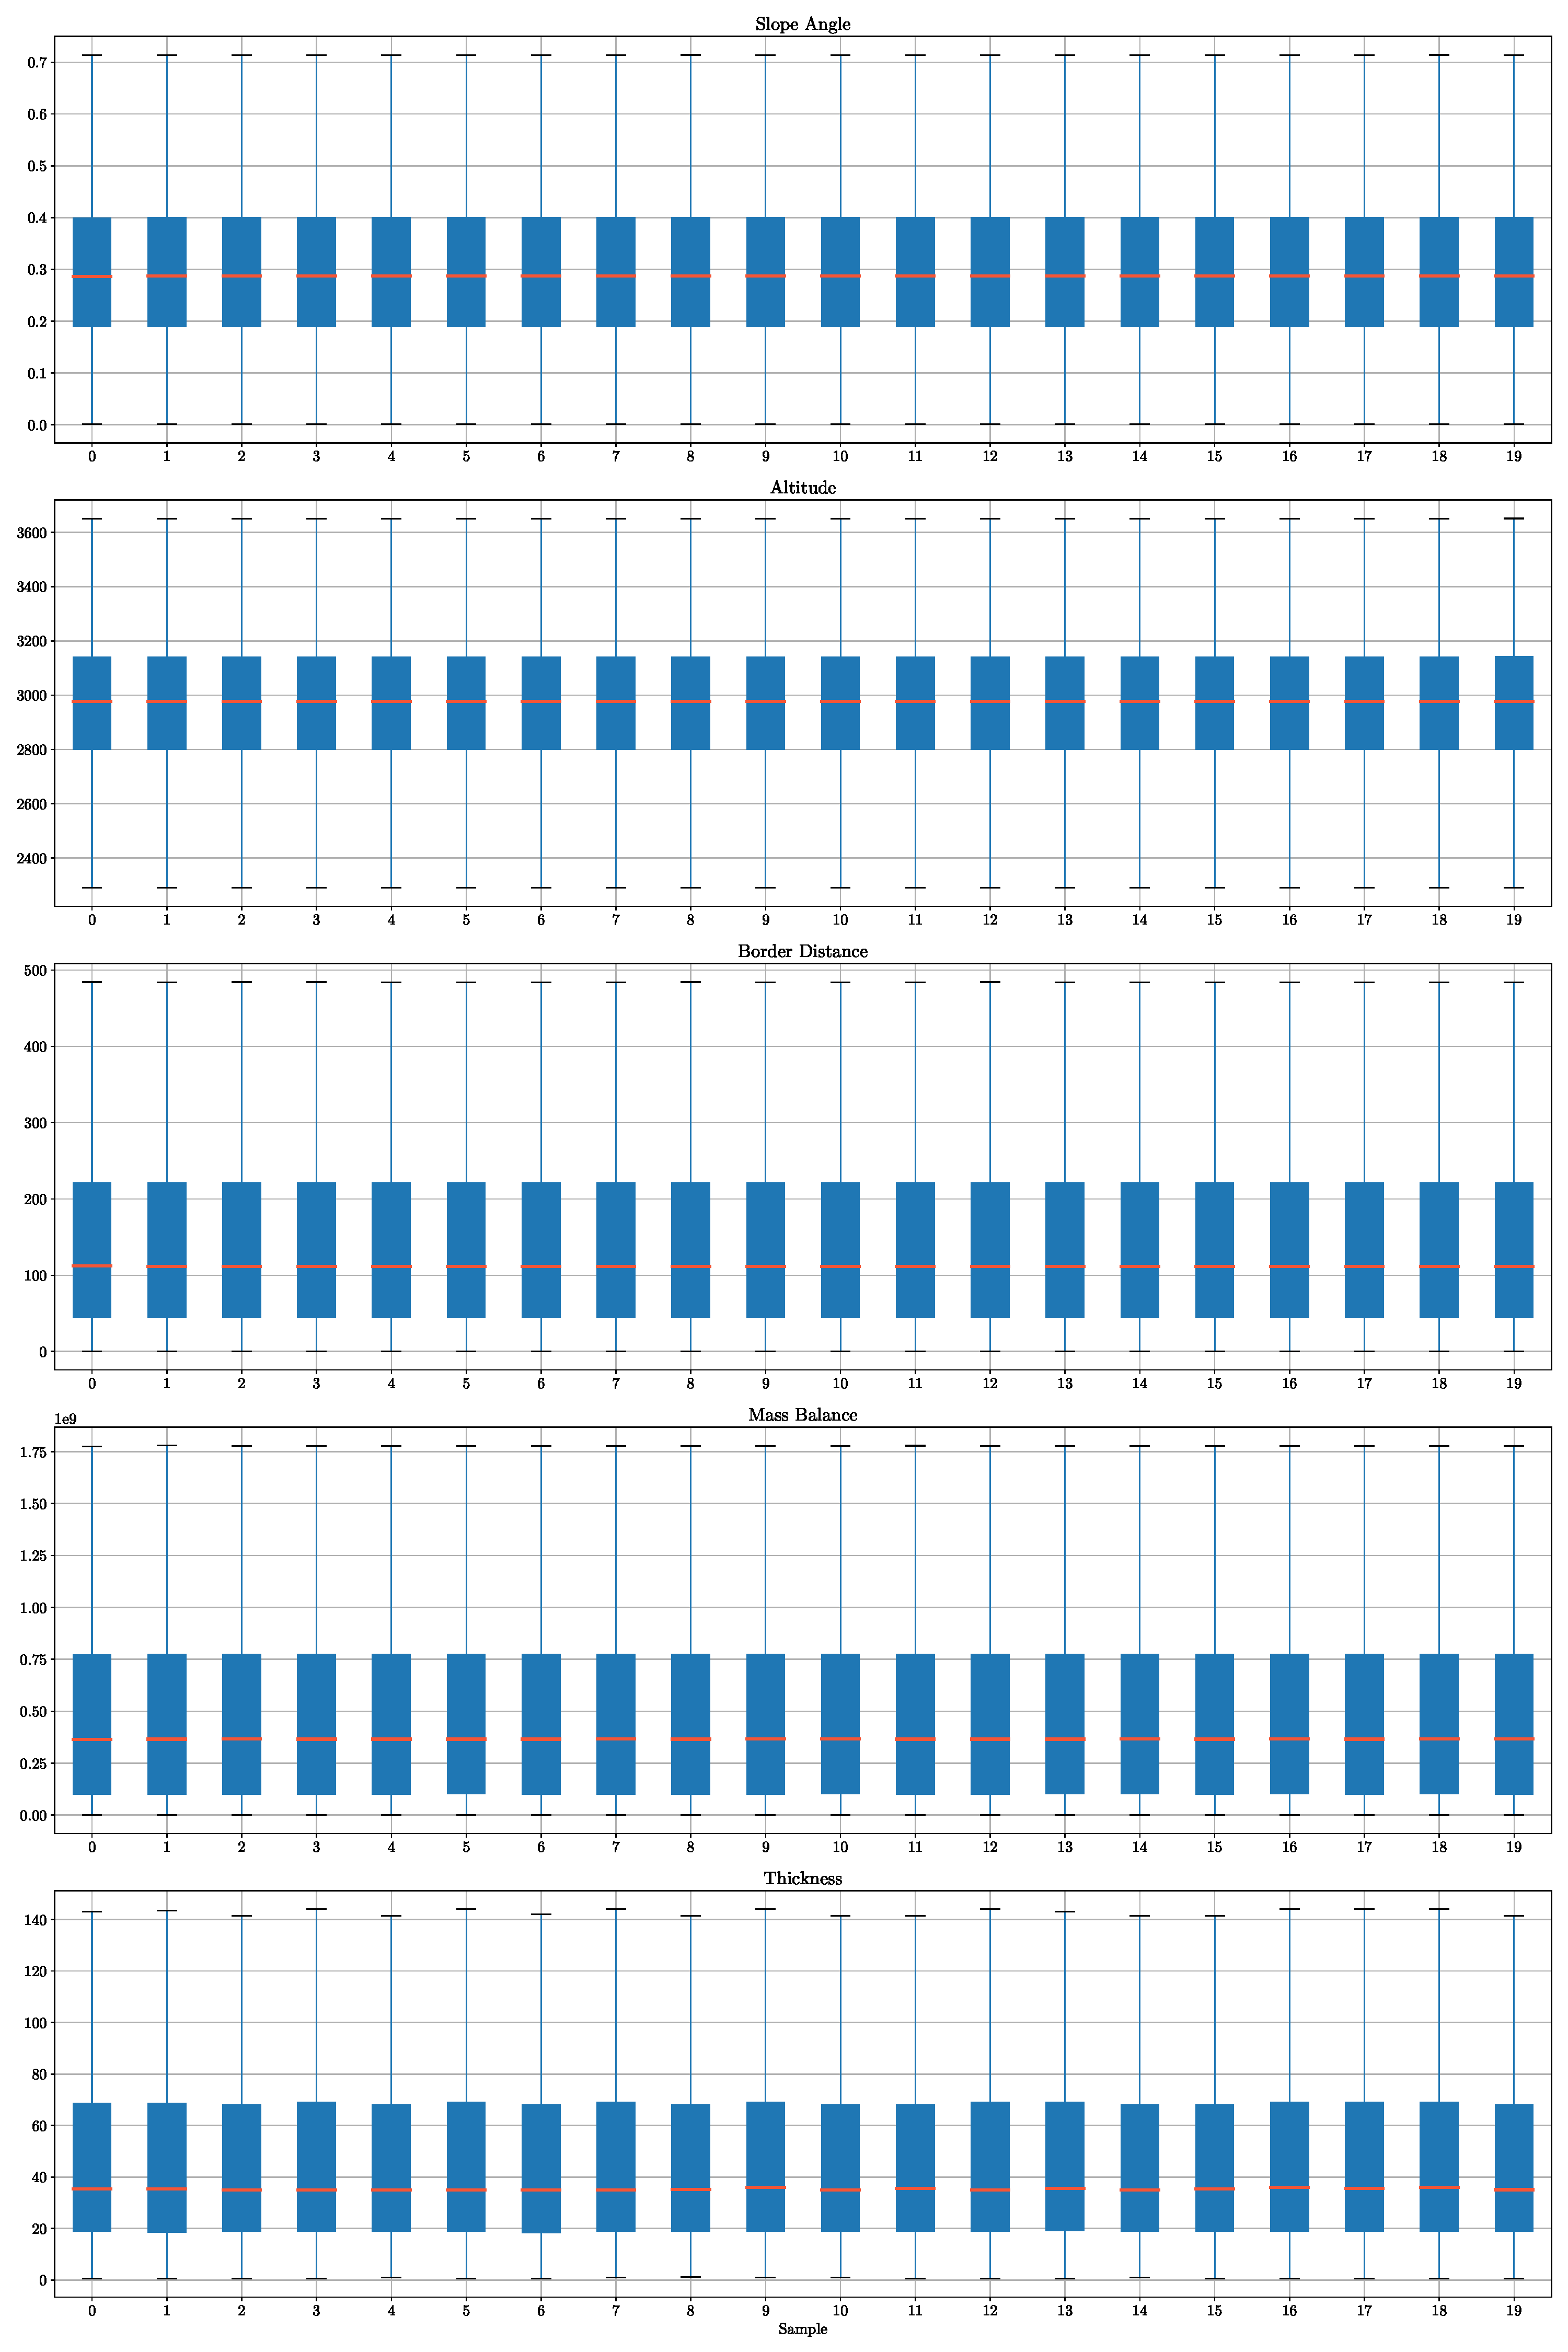
\includegraphics[width=1.\textwidth]{figures/samples_distribution.pdf}
	\caption{Distribution of the attributes used for training the models along the different sub-samples}
	\label{fig:distribution}
\end{figure}

\subsection{Score}\label{disc-score}

One of the easiest approaches to infer the reliability of a model is to check how good the model is at predicting known values. To do that for a model trained from a machine learning algorithm, one needs to be careful at not over-fitting the model, i.e. having a model which is very good at making predictions for data points coming from the data used to train the model, but very bad at predicting values for data not used for training. For this reason the models have all been trained using 20 different sub-samples and checking  how good they were doing, when making predictions using data left out from the sub-samples used for training.
None of the three models used seem to do a very good job at predicting the ice thickness based on their scores. At best, in fact, the support vector regression had an average score of 0.55 but with a high variance due to sub-samples 5, 14 and 19 having a much lower score. Even the best performing of the trained models, which was one of the support vector regression models, had a score only just above 0.6. This means that the best model explains only 60\% of the variance of the thickness observations in GlaThiDa database.

\begin{figure}[!tp]
	\centering		  
	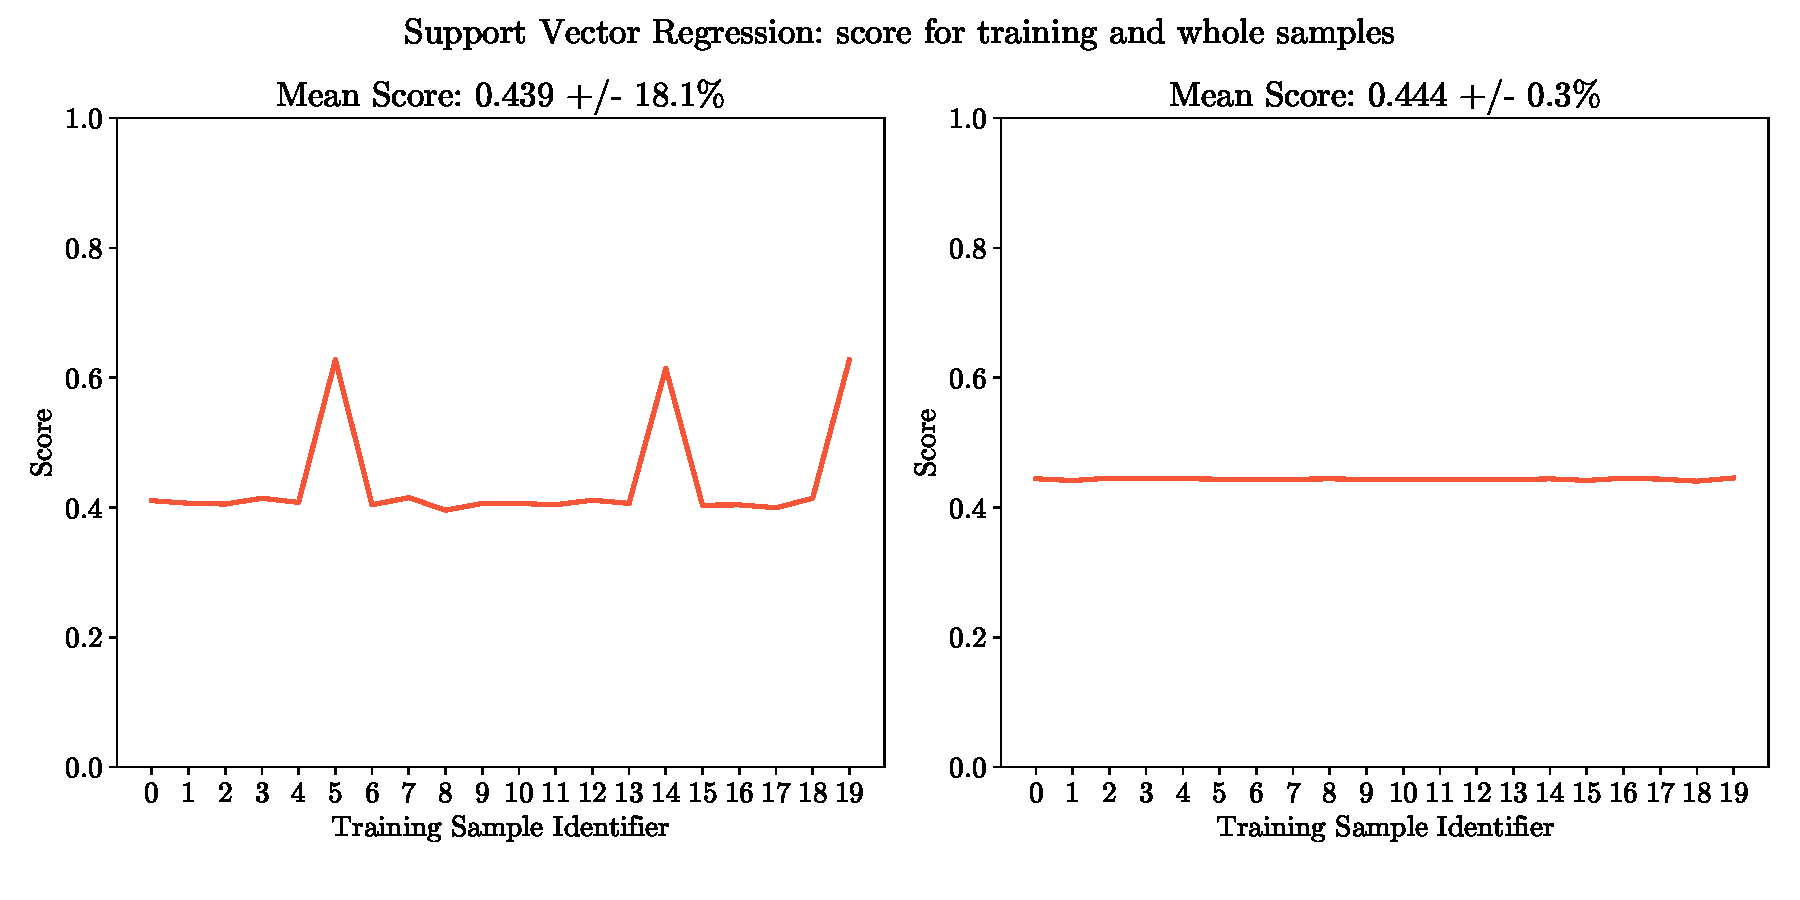
\includegraphics[width=1.\textwidth]{figures/SVR_score_tr.pdf}
	\caption{Support Vector Regression: on the left score achieved by the models trained with the different sub-samples calculated using the training sample instead of the testing sample; on the right the scores computed on the whole sample (train and testing data)}
	\label{fig:train-score}
\end{figure}

Interestingly all the models have drops in performance for the sub-samples  5, 14 and 19. A possible explanation of this behavior could be the fact that the sub-sample used for training these models could be missing some data points, which were essential for training that model, leading to inaccurate predictions. If, for example, those sub-samples had a very different value distribution in any of the attributes used for training, compared to the distribution of the whole data-set, it could lead to biased models not capable of making accurate predictions. This however doesn't seem to be the case when looking at Fig. \ref{fig:distribution} showing box-plots of the data distribution for each of the attributes and sample. No sample, in fact, seem to show a particularly different distribution for any of the features.

\begin{table}[!b]
	\centering
	\caption{Score for the three models used when training them with all the data available from the GlaThiDa.}
	\begin{tabular}{|c|c|c|c|}
		\hline 
		Linear Regression&Random Forest&Support Vector Regression \\
		\hline
		0.32&0.57&0.45 \\
		\hline
	\end{tabular}
	\label{tb:all-score}
\end{table}

Fig. \ref{fig:train-score} shows the score achieved by the support vector regression models, trained with the different sub-samples. On the left the score was calculated only on the sample used for training. This shows a contrast with the results shown in Fig. \ref{fig:svr-score}, which showed the score computed on the data not used for training each sub-sample: the highest scores showed in Fig. \ref{fig:train-score}, are in fact achieved for sub-samples 5, 14, and 19. Those are the same sub-samples which were showing the lowest scores when computing the score only on the testing samples. On the right we can see the scores computed on the whole data-set for the models trained with the different sub-samples. The scores are almost constant throughout the sub-samples. All this could be indicating that the reason for the drop in scores showed in chapter \ref{chap3}, could be attributed to the fact that the samples left out for testing in sub-samples 5, 14 and 19, are particularly difficult to compute for the model. Similar results can be shown also for the linear regression model and for the random forest regression.

Even if the random forest model achieved an average score lower than the one achieved by the support vector machine one, when training them with the sub-samples, the score of the random forest regression achieved when training it on the whole sample is the highest among the models used (see Tab. \ref{tb:all-score}). This score is calculated on the same data used to train the model. It could then be prone to over-fitting, in particular for the random forest regression, which already showed some possible signs of this, when looking at the scores for the different sub-samples.

\subsection{Volume Distribution}\label{disc-vol-dist}
The score is a great value to assess how well the model replicates known data. For glaciers however, looking at the distribution of the ice thickness over the glacier surface in a map is also important. Clearly both the random forest and the support vector regression models have problems in computing large values of ice thicknesses as showed in Fig. \ref{fig:rfr-map} and Fig. \ref{fig:svr-map}. For the random forest regression it seems that there is a an upper ice thickness threshold after which the model computes a constant ice thickness value. This is why the ice thickness distribution maps show large zones of constant ice thickness towards the middle of the glaciers. This can also be confirmed when looking at Fig. \ref{fig:rfr-pdp} which shows that, after a certain threshold, the model predicts no ice thickness change for any change in any feature value. This is clearly a downside of this model which can only predict values within the range of the values found in the training data-set. To improve the prediction for the model for large ice thickness values one could increase the maximum depth of the trees and the minimum number of samples needed for splitting at the node. This would make the model able to better distinguish values for outliers. However there will always be an upper and lower limit for values predicted by the model.

\begin{figure}[!tp]
	\centering		  
	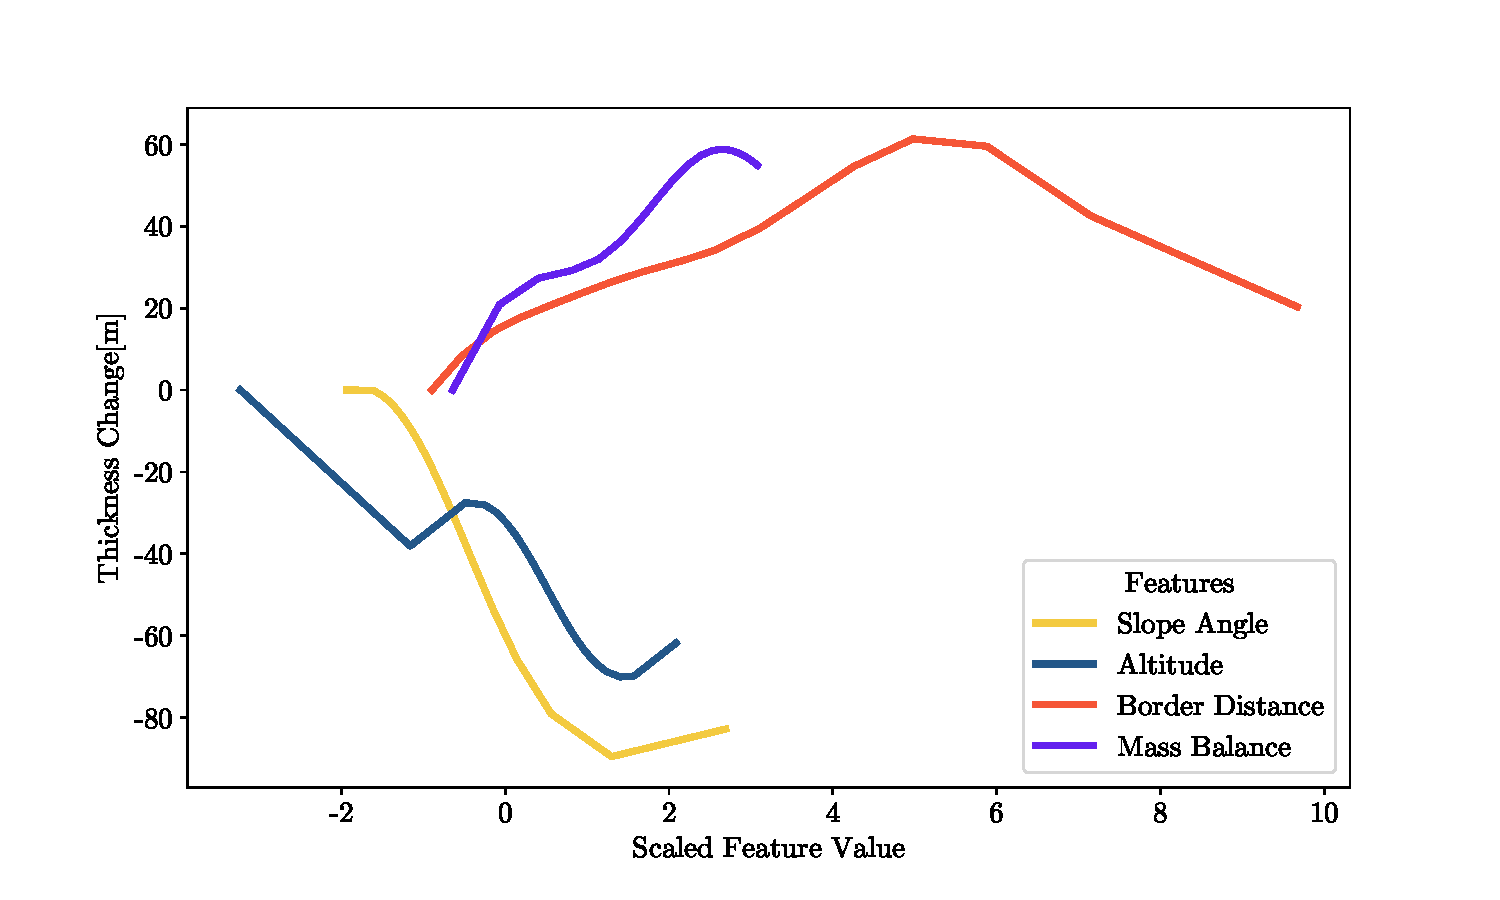
\includegraphics[width=1.\textwidth]{figures/SVR_low_thick_pdp.pdf}
	\caption{Partial plot analysis for glacier RGI60-11.01450 as predicted by the support vector regression model. The chart shows the change in ice thickness dependent on the change in values in the features used for training.}
	\label{fig:svr-pdp-low-thick}
\end{figure}

The support vector regression model presents a different problem when predicting the ice thickness distribution for some glaciers, as for instance RGI60-11.01450, which is a glacier with no thickness observations, hence not used for training the models. The model seems unable to predict a reasonable ice thickness value and its distribution for this glacier. In particular the thickness value predicted for the glacier seems to be too small for such a large glacier and it is constant almost over the whole glacier. The reason for this is probably the fact that, for this particular glacier, the linear mass balance greatly exceeds any value found in the training data-set as one could argue looking at Fig. \ref{fig:svr-pdp-low-thick}. This shows the partial dependence plot for the predictions of the support vector regression model for the input data for glacier RGI60-11.01450. Comparing it to Fig. \ref{fig:svr-pdp}, found in the results, showing the partial dependence plots for data inside the training data-set, and looking at the maximum values reached by  the linear mass balance for both cases, it's clear that for RGI60-11.01450 this feature reaches much larger values. The model then has no way of knowing how to behave for such values as they are completely out of what it "learned" from the training process. Furthermore Fig. \ref{fig:svr-pdp} shows that the model learned that, after a certain threshold for the linear mass balance, the ice thickness decreases. An similar but amplified behavior, is visible for glacier RGI60-11.01450, which led to ice thicknesses much lower than expected. After this decrease the model predicts no further ice thickness changes, as it had been trained with no information about linear mass balances as high as those reached for RGI60-11.01450. This leads to a constant, low ice thickness distribution across the whole glacier.

Overall the performance of the predictions from the models doesn't seem to replicate the available observations in a particularly accurate manner. One of the causes for this, together with what already mentioned, could also be the temporal gap between when the observations were taken, which as seen in section \ref{survey-year}, has a rather high variance, and when the digital elevation model used to compute the features was compiled; glacier flows transform the glacier surface rather fast, and thickness observations taken in one year could look rather different a couple of years later. Digital elevation models and observations measurements represent a single snapshot in a specific time and if the temporal gap between the ice thickness observations and these snapshots was lengthy, the relationship between the geometrical features derived from the digital elevation model and the ice thickness, could be compromised, leading to poor training and predictions.

Also the accuracy of the observations in the GlaThiDa has not been taken into account, and all the observations have been taken as if they were representing the true value for the ice thickness. Errors in ice thickness measurements could potentially be influential in the training process of the models. 

\subsection{Feature importance}\label{disc-features}
For all models the most significant features when making predictions are the slope angle and the mass balance which was expected. However for the linear regression the most influential feature is the slope while for the support  vector machine is the mass balance. For the random forest regression the mass balance also seems like the most relevant feature when looking at the partial dependence plots (see Fig. \ref{fig:rfr-pdp}) and the permutation importance while the default feature importance accessible when training the model suggests the slope to be more influential in making the prediction.

When confronting the permutation importance heat-maps of the 3 models all of them present a drop in the coefficients for the sub-samples 5,14 and 19. This could be explained by the fact that the training data used in those sample are lacking information needed for the model to learn and therefore the importance of each feature used being lower. However recalling Eq. \ref{eq:perm} the permutation importance coefficient is the reduction in the score of model when preforming the permutation on the feature. As the score for the sub-samples already was low this reduction in score was probably less pronounced for those sub-samples. 

Finally looking at the partial dependence plots for the three models, non linear behavior of random forest and support vector regression, are clear. This can be an advantage of course when dealing with non linear dependencies. However while the linear model is able to predict any value even if completely out of the range of values used for training, the other two seem to struggle with those values. This doesn't mean that the linear model would necessarily lead to better prediction for those values but it shows how important is the training data-set for the other models. The best possible solution would be to train those models with data covering all the possible ranges of inputs and outputs.

\section{Alps volume comparison}\label{disc-alps}
A final interesting question is how the models used in this thesis compare with the model proposed by \citet{Farinotti2019} (ITMIX) which uses an ensemble of 5 physically based glacier models to model the glacier ice thickness of all glaciers in the world. The interesting comparison is that while those models are based on physical assumptions and  equation to predict the ice thickness, no assumption has been made in order for the machine learning models to make their predictions aside for choosing which input data to use to train them.
 
The data from \citet{Farinotti2019} comes as a list of all the glaciers with associated glacier volume as predicted by the ensemble of models. It is then possible to get an estimate of glacier ice volume for the whole world.
In order to keep thing simpler when training the machine learning models, the comparison has only been held for glaciers in the alpine regions and with the deletion of 36 glaciers for which it wasn't possible to compute the glaciers attributes needed for training.

\begin{table}[!tp]
	\centering
	\caption{Alpine glaciers total ice volumes in $m^3$ as predicted by the models. Differences are referred to the model from \citet{Farinotti2019} with the experiment called ITMIX}
	\begin{tabular}{|l|c|c|c|c|} 
		\cline{2-5}
		\multicolumn{1}{l|}{}                                                  & ITIMIX              & Linear Regression      & Random Forest           & Support Vector  \\ 
		\hline
		Volume [$m^3$]                                                                & 1.28$\times10^{11}$ & 1.40$\times10^{11}$    & 9.61$\times10^{10}$      & 9.58$\times10^{10}$        \\ 
		\hline
		\begin{tabular}[c]{@{}l@{}}Volume Difference\\from ITMIX [$m^3$]\end{tabular} & -                   & 1.25$\times10^{10}$    & -3.21$\times10^{10}$    & -2.82$\times10^{10}$      \\ 
		\hline
		Volume Difference \%                                                   &                 -    & 9.81\% & -22.1\% & -25.1\%   \\
		\hline
	\end{tabular}
	\label{tb:disc-vol}
\end{table}

The comparison table \ref{tb:disc-vol} shows the total volumes of ice for glaciers in the alpine region computed with the different machine learning models compared to the model from ITMIX. The linear regression model predicts the highest volume while the support vector regression predicts the lowest. Both random forest and support vector regression predict a total volume lower than the one predicted from ITMIX by over 22\%. These two models potentialy underestimate the total volume of alpine glaciers by over $\frac{1}{5}$ of the total ice volume. This difference is so big that it would make a very high impact in predicting, for example, see level rise especially if those differences were carried through for other glacier regions.

The reason for this discrepancies can be probably be imputed to the large spread in glacier sizes and attributes. The first important thing to notice is that according to the findings of \citet{Farinotti2019} 477 of the examined glacier in the alps are major outliers in the data-set when looking at their volume. In particular this means that these 477 glaciers have volumes larger than three times the inter-quartile volume range of all the alpine glaciers examined. This means that the vast majority of the glaciers in the alps are predicted to have much lower volumes compared to the largest glaciers. This makes correctly predicting the volume for these large glaciers extremely important when computing the total ice volume for the alpine glaciers. 477 glaciers represent the 12\% of all the alpine glaciers. According to ITMIX these 477 glacier account for 91.5\% of the total ice volume! Of these 477 glaciers 71 have at least one thickness observation in GlaThiDa which is 67\% of all the glaciers used for training the machine learning models. In theory then the training data-set is potentially well suited to learn about the glaciers with large volumes.  

\begin{figure}[!tp]
	\centering		  
	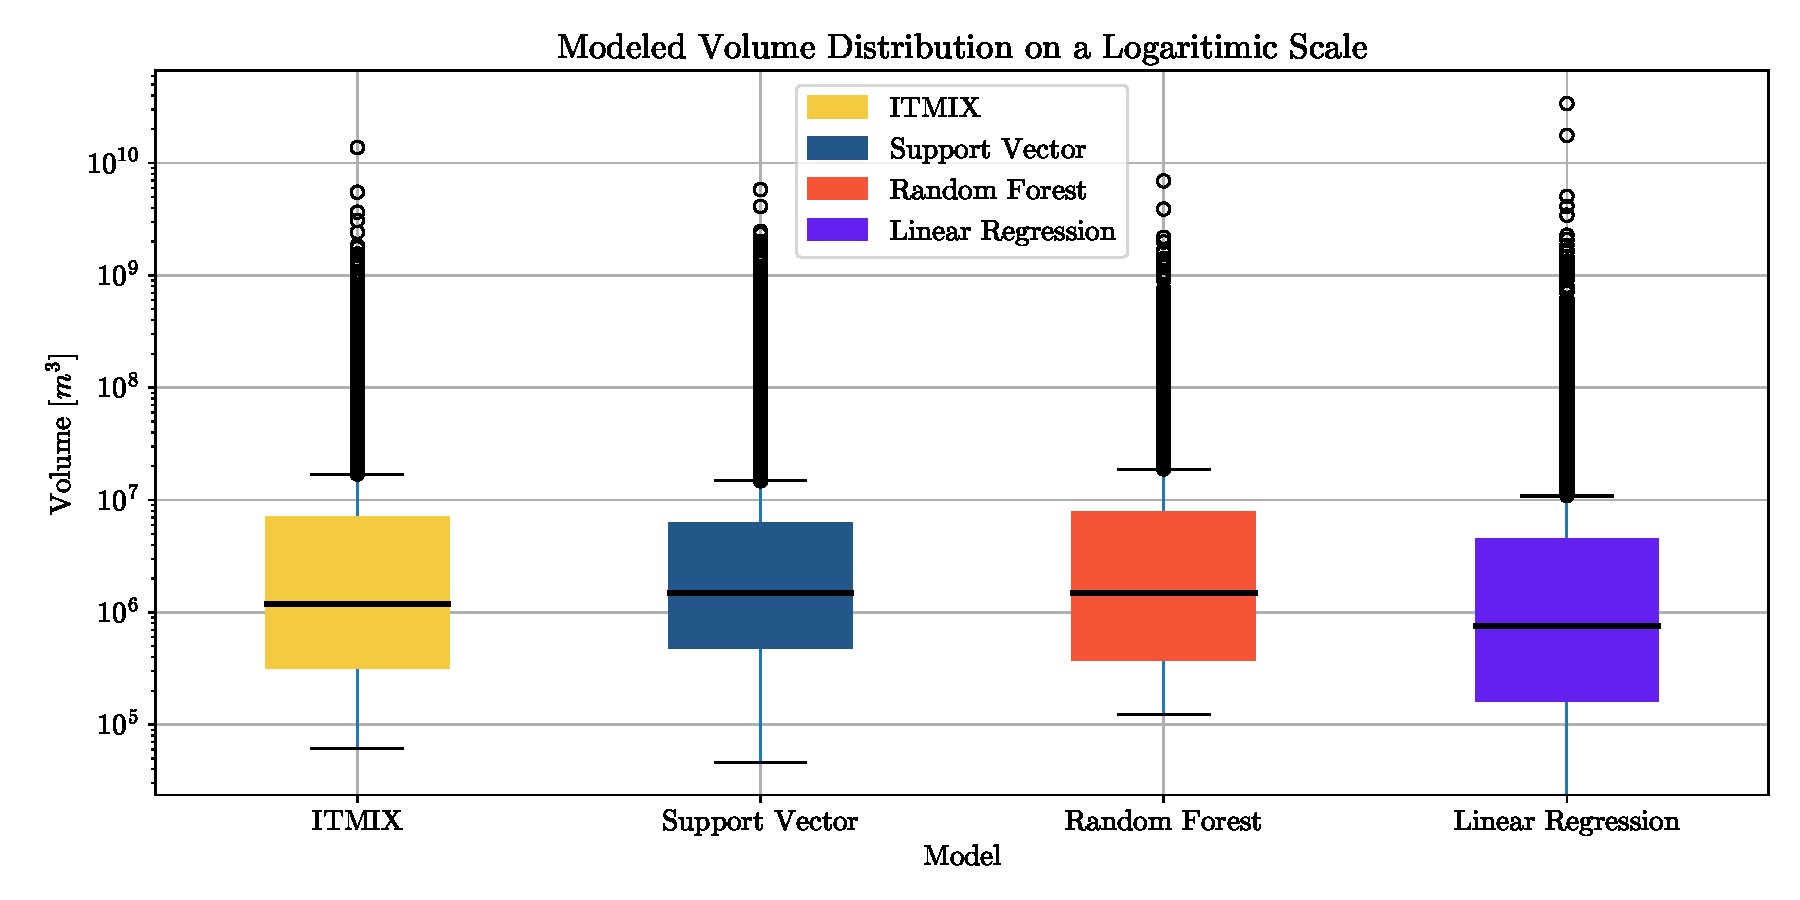
\includegraphics[width=1.\textwidth]{figures/vol_box.pdf}
	\caption{Distribution of alpine volumes as predicted by each model; note that the \textbf{y-axis is shown on a logarithmic scale}}
	\label{fig:vol-dist}
\end{figure}

Fig. \ref{fig:vol-dist} shows the volume distribution as predicted by all the models where the y-axis has been drawn on a logarithmic because of the large difference in volumes between smaller and larger glaciers. It is clear from the figure that both random forest and support vector regression predict an under-disperse volume distribution for large glaciers whereas the linear model predicts far larger volumes than the ITMIX for some glaciers. The support vector regression seems to have make more disperse predictions for smaller size glaciers while the random forest regression seem to have the lowest spread of all models.
random forest and support vector regression not being able to predict the ice thickness of large glaciers seems then to be the main cause for the differences in volume predictions between these two models and the one from \citet{Farinotti2019}.
The reason for this could be that larger glacier are underrepresented in the training data-set. However as just seen before this doesn't seem to be the case as 66\% of this data-set is composed by glaciers which are predicted to have large volumes.
Another reason could be that the number of observations with high ice thickness in the training data-set is low compared to the number of observations with lower ice thickness. The machine learning model would learn to predict better lower ice thickness than higher ones and it would be biased into predicting those. This is of course a normal behavior as machine learning models are not made to predict most of the data right and not the outliers. This is particularly evident for the random forest regression when looking at Fig. \ref{fig:rfr-map} where clearly the model is unable to predict ice thicknesses higher than 130$m$.
For the support vector regression though this is not necessarily the case as it seems like the model is able to predict ice thickness on the upper end of the ones found in the training data-set. However the model seems to be unable to predict a reasonable ice thickness and ice thickness distribution for some kind of glacier like RGI60-11.01450 as visible on the right of Fig. \ref{fig:svr-map}. As mentioned in section \ref{vol-dist}, this could be due to the fact that the input data used to make predictions fed to the algorithm while training don't fully represent the range of the ones found outside of them. This is clearly the case at least for the mass balance which also was the most influential feature in making predictions. Thirteen glaciers in the alps in fact are computed to have at least some mass balance values above the maximum one found in the training data-set. These thirteen glaciers alone account for almost 30\% of the total volume of the alpine glaciers and none of the models was trained to deal with this data. The total difference between the volume computed in the ITMIX and the one computed by the support vector regression for these thirteen glaciers, makes up almost 35\% of the total difference between the two models. 
Clearly not having the whole spectrum of possible input and output values available for training undermines the capability of making predictions of the machine learning algorithm. In this particular case this problem is enhanced by the fact that those values are the most important to the final result as of course bigger glaciers with higher ice thicknesses are the ones which most affect the total volume. 


%The discussion is the interpretation and evaluation of the results. It is a
%comparison of your results with previous findings. It provides the answer to the
%scientific questions raised in the introduction. It is the ``nerve center'' of a
%thesis, whereas the chapter Results may be seen as the ``heart''.
%
%Clearly separate between your own contributions and those of others. Provide
%rigorous citations of appropriate sources! Explicitly refer to specific results
%presented earlier. A certain amount of repetition is necessary. For
%example, the results presented in \ref{3sec:2} suggest that \dots. Order
%discussion items not chronologically but rather logically.
%
%The chapter Results answers the question: \emph{What} has been
%found? (Facts). The chapter Discussion answers the question: \emph{How} has the
%result to be interpreted? (Opinion).
%
%The most important message should appear in the first paragraph. The answer to
%the key question may appear in the first sentence: e.g., did your original idea
%work, or didn't it? The following questions may be answered in the discussion
%section:
%\begin{itemize}
%\item Why is the presented method simpler, better, more reliable than previous
%ones?
%\item What are its strengths and its limitations?
%\item How significant are the results?
%\item How trustworthy are the observations?
%\item Under which precondition/assumption and for which region are the
%results/method valid?
%\item Can the results be easily transferred to other regions or fields?
%\end{itemize}

\newpage
\thispagestyle{plain}


% ==== CONCLUSIONS =============================================================
% ---- set some counters to zero:
\setcounter{equation}{0}
\setcounter{table}{0}
\setcounter{figure}{0}
% ---- include tex-file:
\chapter{Conclusions}\label{concl}
\thispagestyle{plain}

%This chapter contains consequences that derive from your results. It may also
%contain speculations. It may provide suggestions for future studies. Hence, the
%conclusions may provide an outlook and list open questions. Sometimes
%this chapter is part of the discussion. In such a case, the chapter reads
%``Discussion and Conclusions''.

To be decided

\newpage
\thispagestyle{plain}


% ==== APPENDIX ================================================================
% ---- start appendix:
\appendix
% ---- set some counters to zero:
\setcounter{equation}{0}
\setcounter{table}{0}
\setcounter{figure}{0}
% ---- include tex-file:
\chapter{Large Quantities of Data}\label{appA}
\thispagestyle{plain}

Large quantities of data should be placed in an appendix. They should only be
``summarized'' in the chapter Results. Another way is to present
some representative cases together with some extreme cases in the chapter
Results. In any case, there should always appear a reference to the appendix in
the main part of the thesis.

\newpage
\thispagestyle{plain}


% ==== START BACK MATTER (this has no visual effect)============================
\backmatter 


% ==== BIBLIOGRAPHY ============================================================
\addcontentsline{toc}{chapter}{Bibliography}
% ---- use AMS reference format (use file ametsoc.bst included in ...
%      ... http://www.ametsoc.org/pubs/journals/AMS_Latex_V3.0.tar.gz):s
\bibliographystyle{./ametsoc}   % ametsoc.bst in local directory
% ---- use BibTeX database file:
\bibliography{./mybibfile}      % mybibfile.bib in local directory
\newpage
\thispagestyle{plain}


% ==== ACKNOWLEDGMENTS =========================================================
% ---- include tex-file:
\chapter*{Acknowledgments}
\addcontentsline{toc}{chapter}{Acknowledgments}
\thispagestyle{plain}
The idea behind using machine learning was born from my motivation to dive deep into this topic. The idea to use machine learning in relation with glacier modeling however, developed by following a course from Alex Jarosch who had previously participated in the development of the model from \citet{Clarke2009}. A special thanks then goes to him for the inspiration about this work.

The development of this thesis however was only possible thanks to Fabien Maussion, who already had in his mind the idea of using statistical models to estimate glaciers ice thickness from observations. A huge thanks than goes to him, who allowed me to work on the topic i wanted to explore, and gave this work its research focus. He also helped me navigating the hassles of having to deal with geographical data and the tools to do so (OGGM), and guided me through the whole process needed to complete this work. 

On this regard a big thanks goes to the whole OGGM community who made this thesis possible with the creation of the OGGM model.

Thanks also to Reto Stauffer who helped with focusing the statistical part in the right direction.
\newline

Thanks to all the friends i met during these years of studies at the department of atmospheric sciences and in particular to: Antonio, Edoardo, Mattia and Riccardo.

Thanks to Kata and Luigi who encouraged me to start this master course during a climbing day!
\newline

I would then like to thank my family and in particular my mom who helped me correcting the grammatical part of the thesis. 

A final huge thanks goes to my wife Cristina who supported me through the whole process of this master course and made studying for me these years possible. She is the one without whom writing this thesis wouldn't have been possible. It's been wonderful writing it with you and Isabella by my side! Having you made this work a type 2 experience and made the quarantine circumstances of the covid-19 a very happy time for me.

%Now it is time to thank all people who have contributed to your work and who
%have supported you during your study. Do not forget to mention all relevant data
%providers and funding agencies (also provide the grant numbers).

\newpage
\thispagestyle{plain}


% ==== CURRICULUM VITAE ========================================================
% ---- include tex-file:
%\chapter*{Curriculum Vitae}
\addcontentsline{toc}{chapter}{Curriculum Vitae}
\thispagestyle{plain}
%
%
% ---- name, address, and date of birth:
\vspace{-0.5cm}
FirstName LastName\\
Address\\
Born on 01 April 1976 in Town, Country
\\[5mm]
%
%
% ---- education:
\textsc{Education and Professional training}:
\\[1ex]
\begin{tabular}{@{} p{2.5cm} @{} p{12.5cm} @{}}
1999--2003 &
Research assistant and Ph.D. student in the group of Dr. LastName at the
Institute of Meteorology and Geophysics, University of Innsbruck. \\[1ex]
1998--1999 &
Diploma thesis under the guidance of Dr. LastName,
Institute of Meteorology and Geophysics, University of Innsbruck:
\textit{``Title of your diploma thesis''}. \\[1ex]
1993--1998 &
Diploma study at the University of Innsbruck.
\textit{Master of Natural Science (Magister rerum naturalium)} in Meteorology.
\\[1ex]
1989--1993 &
Highschool, Town. \textit{Matura}.
\end{tabular}
\\[5mm]
%
%
% ---- training courses:
\textsc{Meteorological training courses}:
``Numerical methods and adiabatic formulation of models'', ECMWF, 1998; ``Data
assimilation and use of satellite data'', ECMWF, 1998.
\\[5mm]
%
%
% ---- field experiments:
\textsc{Participation in field experiments}:
Gap flow study (MAP), Austria, 1999.

%\newpage
%\thispagestyle{plain}
%
%
%% ==== EPILOGUE ================================================================
%% ---- include tex-file:
%\chapter*{Epilogue}
\addcontentsline{toc}{chapter}{Epilogue}
\thispagestyle{plain}

%Here is the place where you may want to tell a little story or a fairy tale
%which has some relevance for your thesis, such as ``Once upon a time, \dots''.
%The Epilogue is optional.

%\newpage
%\thispagestyle{plain}


\end{document}
% ==== END OF BODY =============================================================
